%Background image credits:https://commons.wikimedia.org/wiki/File:Hemp_paper_in_Japan.jpg タバコはマーダー, CC BY-SA 4.0, via Wikimedia Commons and Gustave Moreau Public Domain.
\documentclass[landscape, a4paper, 11pt, oneside, polutonikogreek, french]{article}
\usepackage[default]{frcursive}
\usepackage[T1]{fontenc}
% Load encoding definitions (after font package)

\usepackage[dvipsnames]{xcolor}
\usepackage{eso-pic,graphicx}
\usepackage[top=42mm, bottom=50mm, outer=33mm, inner=33mm]{geometry}
\setlength{\columnsep}{90pt}
\usepackage{pdflscape}

\usepackage{textalpha}

\usepackage{listings}
\lstset{basicstyle=\ttfamily}

% Babel package:
\usepackage[french]{babel}

% With XeTeX$\$LuaTeX, load fontspec after babel to use Unicode
% fonts for Latin script and LGR for Greek:
\ifdefined\luatexversion \usepackage{fontspec}\fi
\ifdefined\XeTeXrevision \usepackage{fontspec}\fi

% "Lipsiakos" italic font `cbleipzig`:
\newcommand*{\lishape}{\fontencoding{LGR}\fontfamily{cmr}%
		 \fontshape{li}\selectfont}
\DeclareTextFontCommand{\textli}{\lishape}

\usepackage{booktabs}
\setlength{\emergencystretch}{15pt}
\usepackage{fancyhdr}
\usepackage{microtype}

\usepackage{sectsty}
\usepackage[titles]{tocloft}

\sectionfont{\Huge}
\subsectionfont{\LARGE}
\subsubsectionfont{\Large}

\usepackage{setspace}
\onehalfspacing

% change color of text, example replace all \color{Goldenrod} with \color{lightgray}
\definecolor{myGreen}{RGB}{204, 234, 146}

\makeatletter % change only the display of \thepage, but not \thepage itself:
\patchcmd{\ps@plain}{\thepage}{\color{myGreen}{\thepage}}{}{}
\makeatother

\color{myGreen}

\begin{document}
\bfseries
\pagestyle{plain} % after changing a pagestyle command, it's necessary to invoke it explicitly
\AddToShipoutPictureBG{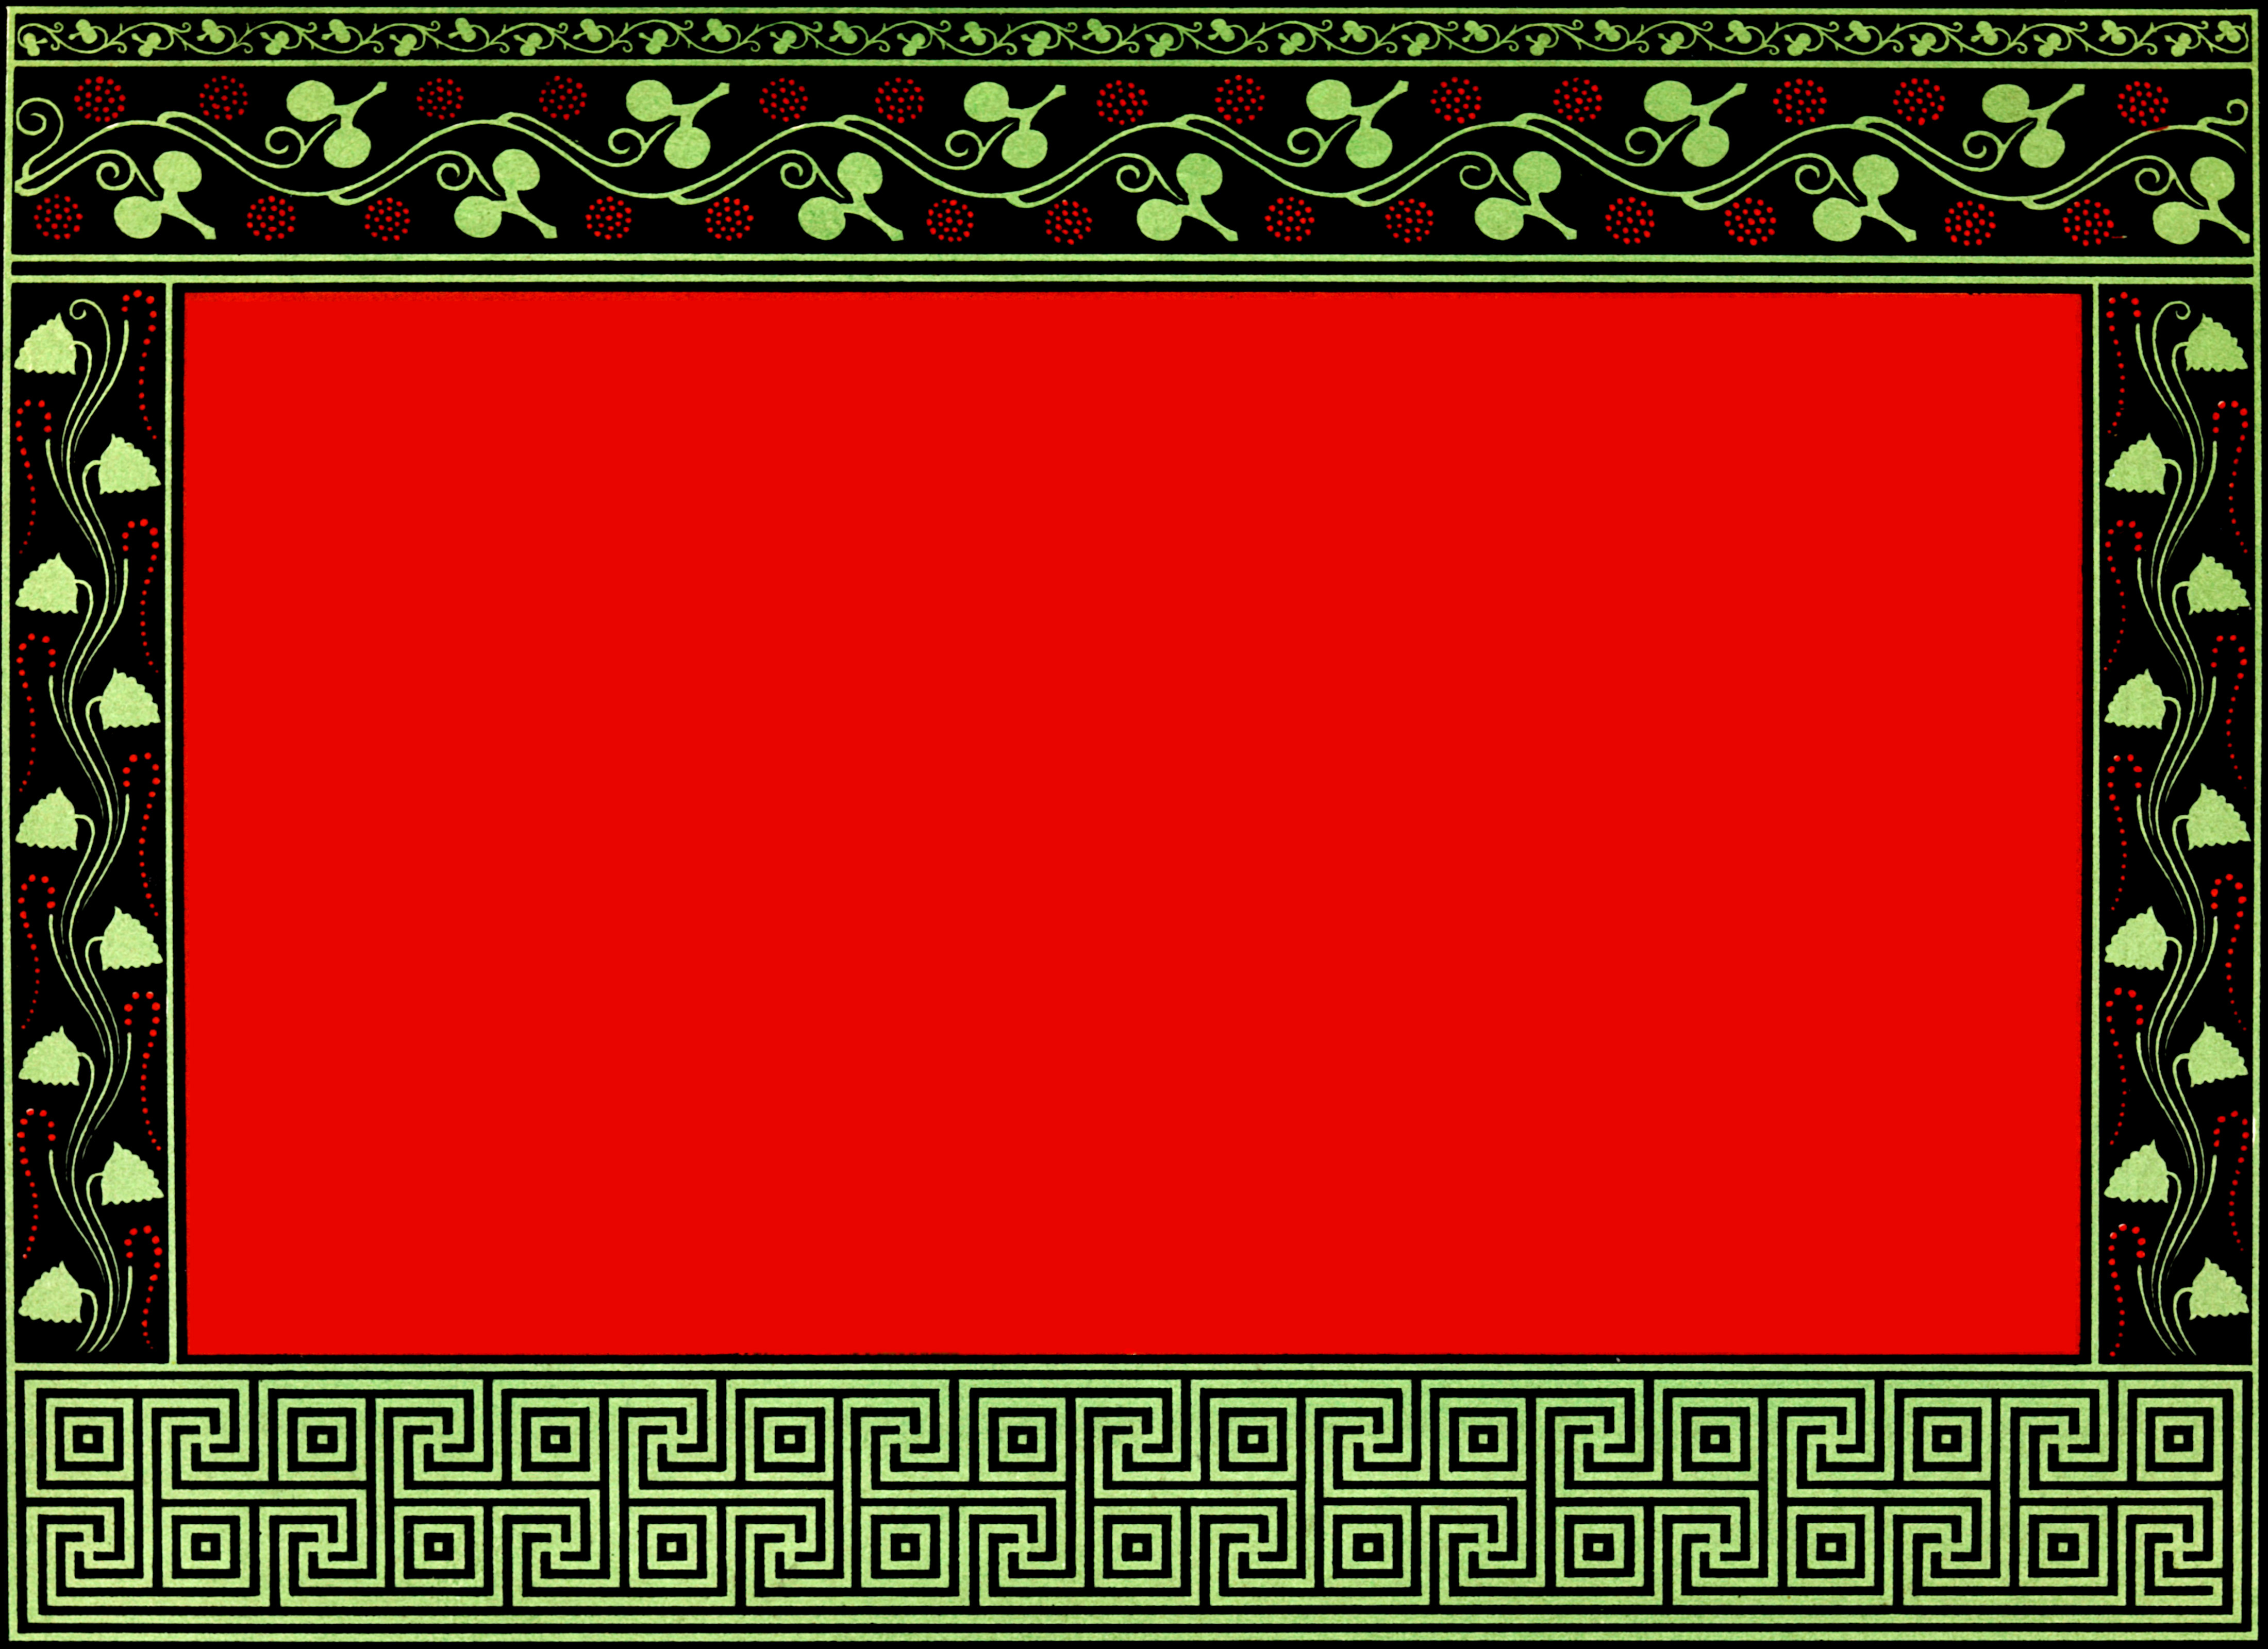
\includegraphics[width=\paperwidth,height=\paperheight]{owens-1.jpeg}}

\renewcommand\thefootnote{{\bfseries\color{myGreen}{\arabic{footnote}}}}
\let\oldfootnote\footnote
    \renewcommand{\footnote}[1]{\oldfootnote{{\bfseries\color{myGreen}#1}}}
\begin{titlepage} % Suppresses headers and footers on the title page
	\centering % Centre everything on the title page
	%\scshape % Use small caps for all text on the title page

	%------------------------------------------------
	%	Title
	%------------------------------------------------
	
	\rule{\textwidth}{1.6pt}\vspace*{-\baselineskip}\vspace*{2pt} % Thick horizontal rule
	\rule{\textwidth}{0.4pt} % Thin horizontal rule
	
	\vspace{1\baselineskip} % Whitespace above the title
	
	{\scshape \Huge Les Muses, \\ Étude de Mythologique Grecque.}
	
	\vspace{1\baselineskip} % Whitespace above the title

	\rule{\textwidth}{0.4pt}\vspace*{-\baselineskip}\vspace{3.2pt} % Thin horizontal rule
	\rule{\textwidth}{1.6pt} % Thick horizontal rule
	
	\vspace{1\baselineskip} % Whitespace after the title block
	
	%------------------------------------------------
	%	Subtitle
	%------------------------------------------------

 	\vspace*{1\baselineskip} % Whitespace under the subtitle

	{\scshape \Large Par Paul Decharme,\\\normalsize Ancien Membre de l'École Française d'Athènes.} % Subtitle or further description

 	\vspace*{1\baselineskip} % Whitespace under the subtitle

	%------------------------------------------------
	%	Editor(s)
	%------------------------------------------------
        \vspace*{\fill}

	\vspace{1\baselineskip}

	{\scshape Paris, 1869. \\\small Ernest Thorin, Libraire-Éditeur rue de Médicis, 7.}
		
	\vspace{0.5\baselineskip} % Whitespace after the title block

        \scshape Internet Archive Online Edition% Publication year
	
	{\scshape\small Utilisation non commerciale --- Partage dans les mêmes conditions 4.0 International} % Publisher
\end{titlepage}
\setlength{\parskip}{1mm plus1mm minus1mm}
\clearpage
\Large
\tableofcontents
\clearpage
\vspace*{\fill}
A M. Egger, Membre de l'Institut, Professeur à la Faculté des Lettres de Paris.

\emph{Hommage de respectueuse reconnaissance.}

\bigskip

P. Decharme.
\vspace*{\fill}
\clearpage
\section*{Introduction.}
\paragraph{}
L'histoire de la religion des Muses, qui est l'objet, de ce travail, commence avec les plus anciennes traditions helléniques, mais ne remonte pas plus haut. L'origine du mythe ne s'y trouve point expliquée : on s'y renferme dans les limites étroites, mais précises, de la Grèce. D'autres diront si les \emph{Apas} et la \emph{Saraswati} des Védas sont réellement les ancêtres des Muses, et si elles peuvent servir à les expliquer. Nous nous bornons à poser cette question, que notre incompétence ne nous permet pas de résoudre.

Dans un sujet ainsi circonscrit et purement grec, la méthode qui s'applique aux études de mythologie comparée ne trouvait point sa place. L'étymologie ne nous a fourni que quelques observations de détail. Pour l'ensemble de nos recherches, nous avons suivi la voie tracée pour la première fois par Ottfried Müller dans ses \emph{Prolégomènes}, et où ont marché après lui tous ceux qui demandent surtout à la Grèce le secret de sa religion. L'appréciation et la comparaison des textes, l'étude des monuments et des diverses représentations figurées, l'observation de la nature grecque, tels sont les éléments que nous avons essayé de combiner et de mettre en œuvre, dans les bornes restreintes de ce sujet.

Le nom des Muses rappelle aux esprits nourris de l'antiquité des images gracieuses qu'on voudrait pouvoir ne pas détruire par les détails d'une étude scientifique. Nous aurons à suivre le développement du culte des Muses, à étudier les variétés de cette croyance aux différentes époques et dans les différentes parties de la Grèce. Les nécessités de l'analyse nous forceront à traiter séparément chacune de ces questions. La pure image des divinités se trouvera nécessairement altérée, et leur chœur harmonieux sera brisé. Comment en serait-il autrement ? On ne saurait prétendre analyser exactement une croyance religieuse antique, et lui conserver en même temps sa vie poétique et son primitif éclat. Pour réunir ce qui a été séparé par l'abstraction, pour donner une apparence de vie à ce qui est mort depuis des siècles, les procédés ordinaires ne suffisent point : il y faudrait une sorte de divination, d'intuition du passé. Cette faculté brillante n'appartient pas à tous ; et qui s'y abandonne sans réserve risque de se laisser égarer, sur un sujet antique, par les fantaisies d'une imagination moderne.

La question qui nous occupe a déjà été plus d'une fois traitée, soit dans les ouvrages généraux qui ont pour objet la mythologie des Grecs, soit dans des dissertations spéciales publiées surtout en Allemagne.

L'histoire des \emph{Religions de l'antiquité} de Creuzer, traduite par M. Guigniaut, les \emph{Religions de la Grèce} de M. Maury, les \emph{Mythologies grecques} de Preller, Welcker et Gerhard, consacrent aux Muses des chapitres que nous avons lus et consultés avec profit. Deux opuscules sur la même question, l'un de \emph{Gyraldi}, l'autre d'\emph{Albertrandi}, ne nous sont point parvenus.\footnote{Des extraits de ce dernier se trouvent dans les \emph{Comm. soc. philol.} de Leipsick, tom. 3, pag. 43 et suiv.} Mais nous avons eu sous les yeux la dissertation de Petersen : \emph{De Musarum apud Græcos origine, numero nominibusque} ; celle de Godefroy Hermann : \emph{De musis fluvialibus Epicharmi et Eumeli}\footnote{\emph{Opuscul.} 2, pag. 288. Cf., Ch. Lenormant, \emph{Élite des monuments céramographiques}, tom. 2, pag. 251.} ; un article de Butmann, dans son \emph{Mythologus}, sur les rapports des Muses avec les Nymphes des fontaines\footnote{Cet article a pour titre : \emph{Mythologische Vorstellung der Musen} (\emph{Mythol.} 1, pag. 275 sqq.).} ; un article de M. Guédéonoff : \emph{Groupes de muses antiques}, dans les \emph{Annales de l'Institut archéologique} (1852) ; enfin la dissertation latine \emph{De Musis}, du docteur Schillbach, l'ouvrage le plus récent sur la matière, et où se trouvent en partie résumés les travaux précédents.

Si, après toutes ces savantes études, il nous a été donné de trouver encore quelques détails nouveaux, c'est au sol de la Grèce et à ses ruines que nous le devons. Le séjour de Rome ne nous a pas été moins utile ; nous avons pu réunir toutes les informations nécessaires à ce travail, grâce à la bibliothèque de l'Institut archéologique, qui a été mise à notre disposition avec la plus complète et la plus aimable libéralité.
\clearpage
\section{Chapitre Premier. --- Les Muses dans Homère et la Théogonie.}
\paragraph{}
Il ne faut pas demander à l'étymologie le sens primitif des Muses. Le nom de ces divinités a été l'objet d'explications nombreuses et très-différentes\footnote{G. Curtius (\emph{Grundzüge der Griech. Etym.}, pag. 280) le rattache au radical sanscrit \emph{man}, en grec μεν ou μαν, d'où μέν-ος, μαν-ία, μέ μον α, \emph{etc.} D'après la forme dorienne Μῶσα la forme éolienne Μοῖσα, Μοῦσα viendrait de Μονσα = Μοντια. Lottner (\emph{Zeitschr.} 6, 109 sqq.) considère ce mot comme équivalent à μάντι-ς ( = μαντι-α). Suivant Th. Bergk (\emph{Lyr. Gr. ad. Pind. Olymp.} 1, v. 15), le nom des Muses vient du mot Lydien μωΰς (\emph{Hésych.} μωῢ, ἡ γῆ, Λυδοί ; lisez πηγή) ou μῶῡ (\emph{Hés.} μῶῡ · τὸ ὕδωρ). --- M. Egger incline à le faire dériver de μῦθος (μοῦθος, fém. μου-θ-α ou μου-σ-α) ; M. Maury (\emph{Relig. de la Grèce}, 2. 476) de μάω, avec le sens d'agitation et de transport prophétique.\\\hspace*{5mm}Mentionnons les étymologies antiques : celle de Platon dans le \emph{Cratyle}, pag. 406, a : τὰς Μούσας τε καὶ ὅλως τὴν μουσικὴν ἀπὸ τοῦ μῶσθαι ; celle de Cornutus (\emph{De Nat. D.} 14, pag. 43) : ἀπὸ τῆς μώσεως, τουτέστι ζητήσεως ; celle de Diodore (4. pag. 150, c.) : ἀπὸ τοῦ μυεῖν τοὺς ἀνθρώπους et la singulière explication de Plutarque (\emph{Moral.} 1, 582, 51) qui fait dériver Μοῦσαι de ὅμου οὖσαι. --- L'explication du stoïcien Cornutus est reproduite par Suidas, v° Μοῦσα · ἡ γνῶσις ἀπὸ τοῦ μῶ, τὸ ζητῶ.} ; mais aucune n'a un tel caractère de certitude qu'on puisse l'adopter en toute sécurité et en tirer de rigoureuses conclusions. Nous devrons donc commencer par faire l'histoire de la religion des Muses, depuis les plus anciens monuments authentiques de la poésie grecque où il en est fait mention, jusqu'à l'époque où leur culte est fixé. Nous rechercherons ensuite, d'après les indices de tout genre que nous fournirons la topographie, les textes, les monuments, quel a été le caractère primitif et naturaliste de cette croyance.

C'est en Thrace, c'est-à-dire en Thessalie et en Piérie, dans les cantons voisins de l'Olympe, que s'est établie d'abord la religion des Muses. Les poètes primitifs, les aèdes, dont la tradition a perpétué le souvenir sous les noms fictifs d'Orphée, de Linus et de Musée, sont souvent désignés comme serviteurs des Muses, Μουσάων θεράποντες. On les considérait aussi comme fils des Muses et d'Apollon.\footnote{Calliope était la mère d'Orphée (V. Schol. \emph{Apoll. Rhod.} 1, 23 ; \emph{Hymn. Orph.} aux Muses, v. 10 ; Apollod. 1, 3, 2 ; Maxim. Tyr. \emph{Dissert.} 37, pag. 439, éd. Davis). De même Ialemos et Hymenaeos étaient fils d'Apollon et de Calliope (\emph{Schol. Pind. Pyth.}, 4, 313).} Ces témoignages nous permettent de supposer qu'à l'origine la poésie grecque fut intimement unie à la religion, et que les plus anciens hymnes furent composés par les serviteurs des dieux. Les premiers prêtres des Muses furent donc en même temps des poètes qui chantèrent les nobles déesses. Ces hymnes primitifs, dont on ne saurait trop déplorer la perte, s'étaient sans doute conservés dans quelques familles sacerdotales ; ils avaient été apportés par les Thraces sur l'Hélicon,\footnote{Ce sont les Thraces, d'après Strabon (10, 3, pag. 404 ; cf. 9, 2, pag. 352, Bibl. Didot) qui ont consacré l'Hélicon aux Muses.} où Hésiode avait pu les entendre. On aimerait à croire que plusieurs des cantiques chantés dans le sanctuaire de Delphes en l'honneur d'Apollon et des Muses avaient cette lointaine origine. Mais aucun texte ne nous permet de deviner le caractère de ces premiers chants, qui sans doute se perdirent d'assez bonne heure, de même que le sanctuaire primitif des Muses dans l'Olympe, celui de Libethrion,\footnote{Le nom du sanctuaire de Libethrion fut transporté par les Thraces, autrement dit Piériens, en Béotie, où la chaîne de l'Hélicon près de Coronée portait le nom de mont Libethrion (Pausan, 9, 34, 4 ; Strab. 9, 2, pag. 352).} n'existait plus qu'à l'état de souvenir à l'époque historique.

C'est sur les sommets de l'Olympe\footnote{\emph{Iliad.} 2, 484 ; 11, 218.} qu'Homère place le séjour des Muses. Mais déjà le culte de ces divinités n'est plus aussi intimement uni qu'autrefois à l'inspiration poétique. La poésie s'est détachée des sanctuaires pour vivre de sa vie propre ; elle est descendue de la montagne sacrée pour se répandre dans le reste de la Grèce. Ce divorce entre la poésie et la religion des Muses nous est attesté par la légende de Thamyris. « A Dorion, dit Homère, les Muses rencontrant, comme il revenait de chez Euryte en Æchalie, le Thrace Thamyris, firent cesser ses chants divins, parce qu'il osa se glorifier de vaincre même les Muses, filles du dieu qui porte l'égide. Les déesses irritées le privèrent de la vue, lui ravirent la divine poésie et lui firent oublier les sons de la lyre.\footnote{\emph{Iliad.} 2, 594, sqq. Hésiode (ap. \emph{Steph. Byz.} v° Δώτιον) plaçait le théâtre de cette légende dans la plaine de Dotis. Sur le même sujet, voir : \emph{Cycl. Fragm.}, ap. Pausan, 4, 34, 7 ; Strab. 8, 3 ; \emph{Mythogr. Gr.}, éd. Westermann, pag. 127-128.} » Ainsi, longtemps avant Homère, la poésie grecque partie de l'Olympe son berceau, avait parcouru le continent et pénétré jusqu'au centre du Péloponnèse, sous la forme de ces aèdes errants dont Thamyris est un des premiers types. L'audace du poète orgueilleux qui provoque les Muses semble exprimer la lutte de la poésie indépendante et purement humaine contre l'art religieux et sacerdotal des âges primitifs.

Les poèmes homériques ne nous donnent que peu de renseignements sur les Muses. Habitantes de l'Olympe, pendant les festins des immortels elles chantent en alternant de leur belle voix, tandis qu'Apollon tient la lyre\footnote{\emph{Iliad.} 1, 604-605.} ; leurs accents charment les loisirs fortunés de la vie divine. Mais quand le poète les invoque, il semble surtout les considérer comme des divinités de la mémoire. An début du Catalogue, il les appelle à son secours pour savoir les noms de tous les chefs des Grecs ; à la fin du Catalogue, il les prie de lui rappeler quel était le plus vaillant de tous ces héros. Au 11e chant de l'\emph{Iliade}, au milieu du récit de la bataille, comme si le souvenir venait tout à coup à lui manquer, il s'adresse aux Muses pour en apprendre quel fut le guerrier qui s'avança le premier contre Agamemnon.\footnote{11, 218.} Instruites de tous les détails des événements passés, les Muses suppléent pour le poète aux défaillances de la tradition, à l'impuissance de la mémoire humaine. Filles de Zeus, les Muses participent à l'ubiquité et à l'omniscience du père des dieux : « Vous êtes déesses, s'écrie le poète, vous êtes présentes à tout, vous savez tout ; tandis que nous, nous n'entendons que la renommée et nous ignorons les choses mêmes.\footnote{\emph{Iliad.} 2, 485-486. Cf. \emph{Æn.} 8, 645 :\\\hspace*{5mm}\emph{Et meministis enim, Divæ, et memorare potestis ;}\\\hspace*{5mm}\emph{Ad nos vix tennis famæ perlabitur aura.}} » C'est à cette science universelle que se borne dans Homère le caractère des Muses. Elles ne sont pas encore des personnes douées d'attributs distincts ; elles composent un chœur illimité et indéterminé. Leur généalogie n'est pas créée\footnote{Homère cite Jupiter comme leur père (\emph{Iliad.} 2, 491 ; \emph{Odyss.} 1, 10 ; 8, 488) ; il ne fait nulle part mention de leur mère. L'hymne homérique à Hermès, v. 429, cite Mnémosyne comme mère des Muses ; mais on sait que cet hymne est très-postérieur à l'Iliade et à l'Odyssée.} ; leur nombre ne paraît pas fixé.\footnote{Les Muses novénaires se trouvent, il est vrai, citées au vingt-quatrième chant de l'Odyssée (v. 60), mais on s'accorde généralement à considérer ce dernier chant comme beaucoup plus récent que les autres. Voir sur ce sujet, et à propos de ce passage, la dissertation de Spohn : \emph{De extranea Odyss. parte}, pag. 43.}

La religion des Muses n'a revêtu une forme précise et ne s'est définitivent constituée qu'en Béotie, autour de l'Hélicon. Leur culte dans cette région remontait à une haute antiquité. Les Béotiens, par une de ces prétentions si chères à la race grecque, disaient que les Muses avaient été pour la première fois adorées sur l'Hélicon par les Aloïdes, Éphialtes et Otos, géants fils d'Iphimedeia et de Poséidon, une des divinités béotiennes primitives.\footnote{Pausanias (9, 29) tire cette tradition d'une citation de l'\emph{Atthide} d'Hégésinoos, empruntée à l'ouvrage de Callippos le Corinthien sur les Orchoméniens. Les œuvres d'Hégésinoos étaient perdues du temps de Pausanias.} Le culte des Muses était donc considéré comme autochthone en Béotie.\footnote{D'après la même tradition, les Aloïdes étaient les fondateurs d'Ascra, qui fut le berceau de la poésie héliconienne.} D'après une autre tradition, Éphialtes et Otos sont des héros thessaliens envoyés par leur père Aloïos, pour chercher leur mère et leur sœur enlevées et emmenées en Béotie par les Thraces.\footnote{Diodor. 5, 50.} Cette seconde tradition est mieux d'accord avec les témoignages qui nous montrent le culte des Muses apporté par la migration thrace des cantons de l'Olympe dans ceux de l'Hélicon.\footnote{Strab. 9, 2 ; 10, 5.}

Les Muses primitives honorées en Béotie étaient au nombre de trois. D'après les traditions locales, les fondateurs de leur culte furent les Aloïdes, Titans ennemis des dieux.\footnote{Voir leur légende dans Homère (\emph{Iliad.} 5, 385 ; \emph{Odyss.} 11, 304-319). --- Cf. Apollod. 1, 7, 4. Cette légende est béotienne. On montrait à Anthédon (Pausan. 9, 22, 6) le tombeau des Aloïdes et d'Iphimedeia leur mère.} Ils établirent donc la religion des trois Muses, à l'exclusion d'Apollon. A l'âge de neuf ans, arrivés à la hauteur de neuf coudées, les Aloïdes sont tués par le dieu Musagète. Peut-être faut-il voir dans cette légende le symbolisme du triomphe des neuf Muses apollinaires sur la triade thracique. Les Muses ternaires seraient donc originaires de l'Olympe ; le culte des Muses novénaires aurait été apporté dans la Grèce du nord avec celui d'Apollon.

La triade des Muses se rencontra sur le sol de la Béotie avec la triade des Charites, divinités des Minyens d'Orchomène.\footnote{V. O. Müller, \emph{Orchom.}, pag. 177 et suiv.} Peut-être même les deux cultes se confondirent ils à l'origine. Il y eut toujours une relation intime entre ces deux groupes de divinités. Les Charites accompagnent, comme les Muses, Dionysos ; elles font partie, comme elles, du cortége d'Apollon. Dans le grand sanctuaire de Delphes, « Artémis forme le beau chœur des Muses et des Charites ... Ces déesses chantent d'une voix divine Latone et ses enfants immortels.\footnote{Hymn. hom. \emph{à Artémis}, v. 15-20. Cf. \emph{Théogon.} 64 : πὰρ δ' αὐτῇς Χάριτες ... Pindare invoque quelquefois les Charites à la place des Muses (\emph{Nem.} 10, 1).} » Dans l'Olympe, « elles sont assises sur leurs trônes, auprès d'Apollon pythien à l'arc d'or.\footnote{Pind. \emph{Olymp.} 14, 9-10.} » On ne saurait douter que les Charites aient eu primitivement une signification musicale. La statue archaïque d'Apollon Délien, décrite par Plutarque, en est la preuve.\footnote{\emph{De Musica}, p. 1136 a. Pausanias (9, 35, 5) nous apprend que cette statue était l'œuvre des sculpteurs Angelion et Tectaeos, qui vécurent vers la 55me Olympiade.} Le dieu tenait l'arc de la main droite ; sur la gauche il portait les Charites, chacune avec un instrument de musique : l'une avait pour attribut la lyre, une autre la flûte, la troisième la syrinx.\footnote{Ausone (\emph{Idyll.} 11, 30) voit dans ces Charites les trois Muses antiques.} Pindare se souvenait encore du caractère musical de ces divinités, quand il composait son chant de victoire en l'honneur d'Asopichos d'Orchomène.\footnote{Il donne à Euphrosyna l'épithète de φιλησίμολπος, à Thalia celle de ερασίμολπος (\emph{Olymp.} 14, v. 12, 14).} Il est donc possible que les trois Charites orchoméniennes aient été d'abord de véritables Muses ; et la distinction entre ces divinités ne s'est sans doute nettement établie qu'à l'époque où la triade primitive fit place aux Muses novénaires.

Le nombre neuf, généralement assigné aux Muses, s'explique par l'union intime de ces divinités avec Apollon. Il se rattache à un des principaux mythes de la religion apollinaire : la victoire du dieu sur le serpent Python. Suivant la tradition la plus répandue, Apollon, souillé du sang du dragon, avait été obligé de s'enfuir en Thessalie et d'y subir une longue expiation.\footnote{A cette expiation se rapporte la fable de l'esclavage d'Apollon chez Admète.} Il n'était revenu à Delphes qu'après une période de huit années entièrement révolues, ou une \emph{ennéaétèris}.\footnote{Les \emph{Ennéaétèrides} d'Apollon ont un rapport probable avec les observations astronomiques des Grecs et leur calendrier. Voir à ce sujet : Boeckh, \emph{Gesch. d. Mondcyclen der Hellenen}, pag. 10 et suiv. Sur les \emph{Ennéaétèrides} en général : Plut. \emph{Quæst Gr.}, 2 ; Censorinus, \emph{de Die Natali}, 18, 1.} Le culte delphique, qui représentait le combat du dieu, sa victoire, sa fuite, sa purification, rappelait en même temps sa longue absence par l'intervalle qui séparait ses fêtes. Les solennités pythiques ne se célébraient primitivement que tous les neuf ans.\footnote{Schol. \emph{Pind. Pyth. argum.} p. 298, édit. Boeckh.} L'usage des \emph{Ennéaétèrides} était également en vigueur à Thèbes pour les fêtes en l'honneur d'Apollon Isménien.\footnote{Procl. \emph{Chrestom.} ap. \emph{Phot. Bibl.} c. 239.} Les fêtes \emph{Carnéennes} de Sparte, par leur durée et par plusieurs de leurs détails, rappelaient la consécration du nombre neuf au dieu.\footnote{Ces fêtes duraient neuf jours ; on dressait autour de la ville des tentes de feuillage au nombre de neuf, \emph{etc.} (Athen. 4, 19).} Enfin, les Corybantes, fils d'Apollon, étaient neuf.\footnote{Phérécydès de Syros, ap. \emph{Strab.} 10, 472 : Φερεκύδης δ' ἐξ Ἀπόλλωνος καὶ Ῥυτίας Κορύβαντας ἐννέα. D'après une tradition postérieure (Apollod. 1, 3, 4) les Corybantes étaient nés de Thalie et d'Apollon. On connaît les rapports de Corybas, divinité solaire, avec Apollon (Maury, \emph{Relig. de la Grèce.}, 1, 199).} Le même nombre symbolique devait s'imposer au chœur des Muses, dont Apollon était considéré comme chef.\footnote{Varron (ap. August. \emph{De Doct. Christ.} 2, 17) racontait une anecdote inventée par les Grecs pour expliquer le nombre neuf des Muses. Les habitants d'une cité, voulant consacrer dans le temple d'Apollon les statues des trois Muses, avaient mis ces statues au concours entre trois artistes. Les groupes une fois achevés se trouvèrent être d'une égale beauté. La ville, ne sachant à qui donner la préférence, se décida à acheter les neuf statues et à en orner son sanctuaire d'Apollon. De là vint l'habitude de représenter les Muses au nombre de neuf.}

La colonie piérienne qui vint se fixer en Béotie ne se sépara pas, sur cette terre nouvelle, de ses divinités et de ses poètes : les rhapsodes de l'Olympe eurent pour successeurs et pour héritiers les rhapsodes héliconiens, dont Hésiode est pour nous le représentant. Ce furent ces chanteurs qui donnèrent au culte des Muses la forme qu'il devait garder.

Les trois invocations\footnote{Ces trois invocations ont été juxtaposées, probablement à l'époque des Pisistratides, quand on remania les poésies homériques et hésiodiques. Elles ne sont pas du même auteur, et aucune peut-être n'est l'œuvre d'Hésiode. La première (v. 1-36) se rapporte aux Muses héliconiennes ; les deux autres aux Muses olympiques.} qui précèdent la Théogonie nous montrent la poésie de l'Hélicon placée sous l'inspiration immédiate des divinités qui l'habitaient. « Les déesses, dit le poète, m'ont ordonné de célébrer la race des bienheureux immortels, et de les chanter elles-mêmes au commencement comme à la fin.\footnote{\emph{Théog.} v. 33-54.} » Ainsi, chacune des compositions théogoniques ou héroïques des poètes de l'Hélicon était précédée d'un hymne en l'honneur des Muses ; elle se terminait également par l'éloge de ces déesses. Inspirés d'un souffle divin, les aèdes, une branche de laurier à la main,\footnote{\emph{Théog.} v. 30.} allaient chantant les immortels ; mais leurs chants n'étaient que la voix même des Muses toujours présentes. Le culte héliconien grandissait tous les jours et devait bientôt gagner d'autres parties de la Grèce. Déjà les croyances de la race hellénique ont été coordonnées, presque fixées pour l'avenir, et dans ce code religieux, né au milieu des vallées de l'Hélicon, les Muses ont leur place.

Suivant la Théogonie, elles sont nées en Piérie de l'union de Zeus et de Mnémosyne.\footnote{\emph{Théog.} 53, 915 ; cf. \emph{Hymn. Mercur.} 429. Plus tard Himerius (\emph{Orat.} 1, 21) place cette union dans l'Hélicon ; ce qui témoigne de la persistance du culte héliconien des Muses.} Or, Mnémosyne est, d'après Hésiode, une des nombreuses divinités du monde titanique, filles du Ciel et de la Terre.\footnote{Théog. 135; cf. Apollod. 1, 1, 3.} Son union avec Zeus eut donc lieu après la victoire remportée sur les Titans. Plus tard, Pindare racontait que les dieux avaient demandé à Jupiter, vainqueur des Titans, la création de puissances divines capables de chanter ce grand événement et l'ordre nouveau du monde : Jupiter s'était uni avec Mnémosyne, et les Muses étaient nées de cette union. Mnémosyne n'est donc autre chose que le souvenir de la victoire de Jupiter et l'inspiration naturelle qui sortit de l'harmonie et de la beauté nouvelle de l'univers : la création de cette divinité semble se rapporter à l'époque même où fut composée la Théogonie, quand Hésiode, faisant l'histoire des générations successives des dieux, traça le tableau des grandes phases de la création du monde. Dans la suite, Mnémosyne, dont le culte partit d'Éleuthères\footnote{\emph{Théog.} 54 : Μνημοσύνη γουνοῖσιν Ἐλευθῆρος μεδέουσα.} pour se répandre dans les autres cantons de la Grèce, ne fut plus que la mère des Muses, mêlée à leur chœur, honorée et représentée avec elles. La grande idée qu'elle exprime ne se perdit point cependant : les Pythagoriciens et les Stoïciens en avaient gardé le souvenir, quand ils disaient que la puissance de Mnémosyne s'étend à la nature entière, qui, dans ses créations infinies, conserve toujours les mêmes genres et les mêmes formes, et qui produit sans cesse des choses nouvelles, sans oublier les anciennes.\footnote{Porphyr. \emph{Vit. Pyth.} 31 ; Cornut. \emph{De N. D.} c. 17. p. 94 : Μνημοσύνη ἠ τοῦ συναναφέρειν τὰ γεγονότα αἰτία. Voir l'hymne orphique à Mnémosyne. Cf. Lobeck, \emph{Aglaoph.}, p. 731 sqq.}

La généalogie donnée par Hésiode aux Muses, filles de Jupiter et de Mnémosyne, fut celle qui prévalut dans l'antiquité grecque. Il y avait cependant d'autres traditions sur leur naissance. La légende qui leur donne Piéros pour père\footnote{Pausan. 9, 9, 2. D'après une autre légende de basse époque conservée par Apollodore (1, 3, 5), Clio se serait unie avec Piéros, par l'effet de la colère de Vénus à qui elle avait reproché son amour pour Adonis.} indique la provenance de leur culte. Mimnerme,\footnote{Pausan. 9, 29, 4.} Alcman\footnote{Diodor. 4, p. 150 b. Cf. Mnaséas ap. \emph{Arnob.} 3, 37 ; \emph{Schol. Pind. Nem.} 3, 16.} et quelques autres poètes, outre les Muses nouvelles, filles de Jupiter, reconnaissaient des Muses plus anciennes, filles d'Ouranos et de la Terre.\footnote{Cette généalogie se retrouve dans une épigramme d'Antipater de Thessalonique (\emph{Anthol. Jacobs.}, 9, 26, v. 9-10) :\\\hspace*{5mm}Ἐννέα μὲν Μούσας μέγας οὐρανός · ἐννέα δ' αὐτὰς\\\hspace*{5mm}Γαῖα τέκεν, θνατοῖς ἄφθιτον εὐφροσύναν.} Dans cette généalogie, inventée et accréditée par des poètes, il ne faut voir qu'un effort pour exprimer la puissance souveraine des Muses, aussi anciennes que le monde, antérieures même à la royauté nouvelle de Jupiter. Les traditions qui leur donnent pour mère Clymène, nymphe Océanide, ou Antiope,\footnote{Hygin, \emph{Fab.} 1, p. 11, éd. Scheffer ; Cic \emph{De N. D.}, 3, 21, 54.} ou les nymphes \emph{Plusia}\footnote{Les quatre Muses Telxinoè, Aoidè, Archè, Mélétè, étaient, suivant Aratus, filles de Jupiter Æther et de Plusia (Tzetz. ad \emph{Hesiod. Op. et D.} 1).} et \emph{Néda},\footnote{Cic. \emph{De N. D.}, 3, 21.} ne paraissent être que des fantaisies de mythographes. Quand Euripide dit que la blonde Harmonia enfanta les neuf Muses chez les Athéniens,\footnote{Médée, v. 833.} il n'a d'autre intention que de flatter son public. Malgré ces dissidences mythologiques au sujet de la mère des Muses, on peut dire que la croyance des Grecs resta généralement fidèle à la généalogie établie dans la Théogonie.

Les rhapsodes héliconiens fixèrent également le nombre et le nom des Muses.\footnote{D'après Varron (\emph{Fragm.}, éd. Bip., p. 329) c'est Hésiode qui la première donna des noms distincts aux Muses.} Dans la Théogonie, elles sont au nombre de neuf, et elles portent déjà les noms qu'elles conserveront pendant toute la durée de la religion hellénique : Clio, Euterpe, Thalia, Melpomène, Terpsichore, Erato, Polymnia, Uranie et Calliope.\footnote{\emph{Théog.} 76-79.} C'est sous ces dénominations qu'elles furent honorées dans le pays de Thespies, et ensuite dans d'autres cantons de la Grèce. D'après une tradition béotienne recueillie par Pausanias, les Muses primitives, honorées par les Aloïdes, fondateurs d'Ascra, portaient les noms de \emph{Mélétè}, \emph{Mnèmè}, \emph{Aoidè}.\footnote{Pausan. 9 ; 29, 2.} Ces dénominations n'ont pas, sans doute, une si lointaine origine ; elles appartiennent plutôt à une époque de réflexion et d'abstraction, car elles indiquent simplement une division de l'art des rhapsodes en invention, mémoire et chant. Si les Muses ternaires avaient disparu de la religion, leur souvenir s'était conservé dans l'art : on les trouve représentées toutes les trois sur un vase athénien d'époque ancienne,\footnote{Stackelberg, \emph{Gräber d. Hellen.}, pl. 19. On voit Apollon couronné de laurier, assis et jouant de la lyre ; devant lui, Mnèmè qui tient un rouleau de papier, derrière, Aoidè une lyre à la main, et Mélétè avec la double flûte.} et Mélétè se voit avec Musée et Terpsichore sur une amphore de Vulci.\footnote{Cette amphore, actuellement au Musée britannique, a été reproduite dans les \emph{Monuments inédits de l'Institut arch.} de Rome, vol. 5. pl. 37. Cf. \emph{Annales}, 1852, article d'O. Jahn. La légende probablement altérée porte : Τερψιχόρα, Μοσαῖος, et Μελελωσα. Welcker suppose que l'artiste aura voulu écrire : μελετῶσα du verbe μελετάω. Cette Muse serait donc la même que Mélétè. Sa physionomie a une expression sérieuse ; elle est vêtue du simple \emph{chiton} dorique ; elle tient les doubles flûtes, prête à accompagner Terpsichore.}

Fixée dans ses traits généraux par Homère et par Hésiode, la religion hellénique n'eut cependant jamais rien de constant ni d'immuable : elle suivit les caprices de la vive imagination qui lui avait donné naissance ; en passant d'un canton à l'autre, elle se modifia insensiblement, se pliant aux traditions locales et aux fantaisies des poètes. Il ne faut donc pas s'étonner que les Muses novénaires ne soient pas universellement reconnues dans les textes antiques qui nous sont parvenus. D'après certains auteurs, elles étaient au nombre de quatre, allusion probable au tétrachorde primitif.\footnote{Cic. \emph{De N. D.} 2, 21 ; Arnob. 3, 37 : « Ephorus Musas numéro esse tres affert ; Mnaseas quatuor. »} Les sept Muses de Lesbos rappellent l'heptachorde\footnote{Cornut. \emph{De N. D.} 14, p. 47., éd. Osann.} inventé par Terpandre, ou les rapports qui unissent ces divinités à Apollon Hebdomagète.\footnote{Apollon était surnommé ἑβδομαγἐνης ou ἑβδομαγέτης, parce que, suivant les traditions, il était né le sept du mois. On le disait aussi né dans le septième mois de l'année : de là le surnom d'ἑπταμηνιαῖος. Aux fêtes d'Apollon, sept garçons et autant de jeunes filles conduisaient la pompe. Cf. Procul. \emph{in Tim.} 3, 200 ; J. Lydus, \emph{de Mens.} pag. 26.} Le nombre huit, donné aux Muses par les Pythagoriciens, se rapporte, suivant Plutarque, aux huit sphères célestes.\footnote{Plutarch. \emph{Symp.} 9, 14, p. 746 a. On trouve même deux Muses seulement citées dans un passage du stoïcien Cornutus (\emph{De N. D.} 14, p. 47). Mais ces deux Muses sont d'invention philosophique, et de pures allégories. Elles n'ont sans doute jamais existé dans l'ancienne poésie. Telle est aussi l'opinion de Petersen, p. 89 de sa dissertation : \emph{De Musarum apud Græcos origine, numero nominibusque}.} A Sicyone, une des trois Muses portait le nom de \emph{Polymathia}, variante de Polyhymnia.\footnote{Plutarch. \emph{Symp.} 9, 14, p. 746, e.} A Delphes, elles empruntaient leurs noms à l'art de la lyre, comme l'indiquent les dénominations de \emph{Nétè}, \emph{Mésè} et \emph{Hypatè}.\footnote{\emph{Ibid.} 9, 14. p. 744, d.} La religion des Muses fut donc soumise, comme celle des autres divinités grecques, à un certain nombre de variétés locales. Mais tous les témoignages que nous possédons à ce sujet sont d'une époque très-postérieure à la Théogonie, et nous permettent de croire que les Muses distinctes de celles de Thespies n'eurent jamais une grande place ni dans la religion, ni dans l'art. Toutes ces traditions particulières, tous ces cultes locaux, s'effacent pour nous devant le souvenir et les nobles images des Muses héliconiennes chantées par les poètes, vivantes encore dans les monuments de la statuaire grecque.
\clearpage
\section{Chapitre 2. --- Les Muses divinités des eaux.}
\paragraph{}
Les généalogies théogoniques se contentent d'exprimer sèchement le rapport qui unit les Muses aux autres dieux, et de leur assigner une place dans le vaste corps de la religion : elles ne peuvent nous faire soupçonner quelle fut la vie de ces divinités dans la croyance commune. Les Muses n'ont pas été pour les Grecs de pures abstractions. Les premiers poètes, et les plus grands, ont cru à leur existence divine. « Quand Hésiode fait l'éloge des Muses, il n'en parle point par ouï-dire ; il les a vues lui-même.\footnote{Lucien, \emph{De Saltat.} cap. 24. Ces mots, est-il besoin de le dire, ont chez Lucien un sens sceptique. Ils n'en sont pas moins un témoignage en faveur de notre idée. Il est impossible de méconnaître dans le commencement de la Théogonie l'impression d'un sentiment religieux et la trace d'un culte local.} » Les premiers vers de la Théogonie respirent en effet la religion de ces divinités et portent comme l'empreinte de leur présence. C'est dans le pays d'Ascra qu'on entendait pendant la nuit leurs voix harmonieuses, quand, enveloppées d'une nuée épaisse, elles descendaient des sommets de l'Hélicon, chantant les dieux et se communiquant aux hommes ; c'est autour d'Aganippe qu'elles formaient leurs chœurs aimables. Moins présentes dans d'autres cantons de la Grèce, elles y trouvaient cependant un culte et des autels. La vive imagination du peuple croyait les rencontrer au sein des solitudes, dans le voisinage des sources et des eaux limpides. Les Muses étaient alors de véritables personnes, mêlées, comme les hommes, à la grande vie de la nature. Ce sentiment de leur existence divine a dû se conserver longtemps dans les âmes simples, chez les habitants des campagnes, qui, vivant en communication fréquente avec la terre, les forêts et les eaux, en écoutaient tous les bruits, en recueillaient toutes les impressions. Pendant longtemps ils ont cru voir et entendre les Muses dans les endroits déserts qu'elles avaient choisis pour séjours. C'est ce rapport des Muses avec la nature que nous voudrions essayer de trouver.

Le plus ancien sanctuaire des Muses, celui de \emph{Libethrion},\footnote{Pausan. 9, 34, 4 ; Strab. 9, 2, p. 352. Voir le savant travail de M. Heuzey, sur \emph{le mont Olympe}, p. 95.} était situé sur les pentes orientales du mont Olympe. Le nom donné à ce sanctuaire indique qu'il était au milieu d'un pays arrosé et coupé de nombreux ruisseaux.\footnote{Le mot λείβηθρον, qui désigne un canal ou un ruisseau, dérive de la racine λιβ, d'où le verbe λείβ-ω, les substantifs λιβάς, λιβάδιον, \emph{etc.} Voir G. Curtius, \emph{Grundzüge der griech. Etym.}, p. 328.} Les eaux torrentueuses qui descendent de l'Olympe ont en effet, autrefois comme aujourd'hui, donné un nom à ce canton. Les Grecs modernes l'appellent \emph{Canalia}, mot qui traduit exactement l'ancienne dénomination : τὰ λείβηθρα. Ce sont des gorges sauvages, des ravins étroits et profonds, déchirés par les torrents qui roulent avec fracas des pentes supérieures de la montagne ; dans ces profondeurs humides, une puissante végétation est entretenue par l'eau, et de grands sapins s'en élancent pour aller chercher en haut le ciel et la lumière. Bien que la mer et les vastes horizons ne soient pas loin, ici on est enfermé, emprisonné dans une nature sauvage ; on n'y entend que la voix des eaux, les murmures de la forêt, ou la foudre de Jupiter qui tonne sur les sommets. C'est ici que descendaient les Muses, quittant la demeure de leur père, et plus d'une fois sans doute les Piériens qui s'approchaient de cette solitude crurent surprendre la voix même des déesses dans les bruits tour à tour éclatants et harmonieux des torrents. Un autre sanctuaire, celui de \emph{Pimpleia}, leur était également consacré en Piérie. Strabon le place dans le canton de \emph{Dion}, pays humide, aujourd'hui marécageux, revêtu d'épais taillis : le nom de ce sanctuaire\footnote{De πίμπλημι. \emph{Pimpleia} veut donc dire au propre : la source \emph{pleine}.} semble indiquer qu'il était placé près d'une source abondante qui se versait dans un bassin profond, toujours rempli par les eaux.

La colonie piérienne qui vint s'établir en Béotie, y apporta avec elle l'habitude d'honorer les Muses près des cours d'eaux et des fontaines. Le souvenir de la patrie qu'elle avait quittée lui fit donner le nom de Libethrion à cette partie de la chaîne de l'Hélicon qui est voisine de Coronée, et là, près de deux sources « qui ressemblent à des mamelles de femme et versent une eau douce comme le lait, » fut établi un culte des Muses \emph{Libethrides}, qui était encore en vigueur à l'époque de Pausanias.\footnote{9, 34, 4.} Dans la partie de l'Hélicon spécialement consacrée aux Muses, en face d'Ascra, jaillissent de nombreuses sources et courent plusieurs ruisseaux : on connaît les noms d'Hippocrène, d'Aganippe, du Permesse, de l'Olmée ; les ruines du sanctuaire des Muses se voient encore aujourd'hui sur les deux rives d'un torrent.\footnote{Voir notre \emph{Notice sur les ruines de l'hiéron des Muses}, dans les \emph{Archives des missions scientifiques}, tom. 4, 2me série.} A Corinthe, la source de Pégase, Pirène, était consacrée aux Muses.\footnote{Pers. \emph{Sat. Prol.} 4 ; Stat. \emph{Sylv.} 2, 7, 1.} A Trézène, enfin, ces divinités étaient honorées sous le nom de Muses \emph{ardalides}, épithète dont le sens est le même que celui de \emph{libethrides}.\footnote{Plut. \emph{Moral.} p. 150 a ; Pausan. 2, 31, 3. --- Du verbe ἄρδω, mouiller, arroser. Plutarque et Pausanias expliquent ce mot en supposant que le culte des Muses a été établi à Trézène par un certain Ardalos, inventeur de la flûte. Ce procédé commode d'étymologie est trop fréquent chez les écrivains grecs pour qu'il soit nécessaire de s'y arrêter. D'après Pausanias, Ardalos était fils d'Héphaestos, dont le culte à Trézène s'explique par la nature volcanique des côtes de l'Argolide. Héphaestos était également honoré à Epidaure (\emph{Corp. Inscr.} 1179).} Les sanctuaires des Muses étaient donc toujours placés dans le voisinage des sources ou des ruisseaux. Il semble raisonnable d'en conclure que les Muses furent primitivement des divinités des eaux, et qu'en plus d'un endroit de la Grèce elles eurent cette signification pour le peuple. Cette première vraisemblance, tirée de la topographie et de l'étymologie, a besoin d'être confirmée par d'autres témoignages.

Un passage de Tzetzès\footnote{Ce passage est extrait du \emph{Comment. sur les Œuvres et les jours}, pag. 6.} nous apprend qu'Eumélos de Corinthe reconnaissait trois Muses, filles d'Apollon, auxquelles il donnait les noms de \emph{Céphisso}, \emph{Apollonide} et \emph{Borysthénide}. Sans doute on ne peut affirmer que cette citation d'Eumélos soit authentique ; car, dès l'antiquité, les ouvrages attribués à ce poète soulevaient les doutes de la critique.\footnote{Pausanias (4, 33, 3) ne reconnaissait pour authentique, parmi les œuvres attribuées à Eumelos, qu'un \emph{prosodion} composé pour les Messéniens envoyés en mission sacrée à Délos.} Mais, en supposant que le texte cité par Tzetzès dérive d'une source moins ancienne qu'Eumélos, il mérite cependant de fixer l'attention : deux de ces Muses en effet portent des noms de fleuves. Peut-être même, comme le propose God. Hermann, faut-il lire \emph{Achéloïde} au lieu d'\emph{Apollonide}.\footnote{G. Hermann, dans sa dissertation \emph{De Musis fluvialibus Epicharmi et Eumeli} (Opusc. 2, p. 288 sqq.) suppose qu'il s'agit ici d'un mythe analogue à celui d'Apollon Hyperboréen et ses trois frères, fils de Boréas et de Chioné. Eumélos aurait exprimé la même idée d'une autre façon, en substituant les trois Muses aux trois fils de Boréas et de Chioné.\\\hspace*{5mm}Butmann (\emph{Mythol.} 1, p. 273 sqq.) explique ainsi les trois Muses d'Eumélos : Borysthénis, la Muse du nord, rappelle les origines de la poésie grecque et se rattache aux légendes d'Apollon Hyperboréen, d'Orphée, de Linus, \emph{etc.} ; Apollonis est la Muse olympique ; Képhisso, la vraie Muse grecque.} Cette citation nous reporte donc à un culte primitif des Muses sur les rives du Borysthène, de l'Achéloüs et du Céphise ; ou bien, si ces noms sont dus à la fantaisie du poète, ils n'en attestent pas moins la parenté qui unissait le culte des Muses à celui des divinités fluviales.

Un témoignage encore plus précis est emprunté à la comédie d'Epicharme qui avait pour titre : Les \emph{Muses}\footnote{La comédie des Muses, comme nous l'apprend Athénée (3, cap. 75) n'est qu'une édition remaniée des \emph{Noces d'Hébé}.} ou les \emph{Noces d'Hébé et d'Hercule}. « Epicharme, dit Tzetzès,\footnote{\emph{Comment. sur les Œuvres et les jours}, p. 6.} dans le mariage d'Hébé, nomme sept filles de Piéros et de la nymphe Pimpléis : \emph{Nilo, Tritoè, Asopo, Heptaporé, Achéloïde, Titoplo} et \emph{Rhodia}. » On reconnaît facilement que tous ces noms, sauf le mot Titoplo, probablement altéré,\footnote{A Τιτόπλουν God. Hermann substitue Πακτωλοῦν. Cf. Epicharm. \emph{Fragm.} p. 39, éd. Krusemann.} sont empruntés à des fleuves.\footnote{L'Heptaporos et Rhodia sont cités par Homère (\emph{Iliad.} 12, 20) au nombre des fleuves qui descendent des montagnes de l'Ida. Ils sont aussi nommés dans la Théogonie (v. 341).} Mais est-ce par un simple caprice d'imagination que le poète sicilien a appliqué aux Muses ces dénominations ? On sait qu'Épicharme, dans sa comédie des Noces d'Hébé, avait représenté sous des traits ridicules le somptueux banquet des dieux grands mangeurs de poissons, dont Athénée nous a conservé la longue énumération.\footnote{Athén. 3, 30, p. 85, c ; 7, 114, p. 320, c.} Les divinités des eaux se transforment, pour la circonstance, en pourvoyeuses de l'Olympe. Neptune revient avec un navire chargé de coquillages de tonte espèce ; les Muses vont à la pêche en eau douce. De là les noms qui leur sont donnés par le poète. Or, comment Épicharme, dans cette parodie mythologique, aurait-il pu attribuer un pareil rôle aux Muses, si la croyance générale et populaire de son temps ne les avait reconnues comme divinités des eaux\footnote{Sur un vase antique (\emph{Elit. Céram.} tom. 2, pl. 86), on voit un héron aux pieds de Clio : allusion probable au caractère fluvial des Muses.} ?

C'est surtout auprès des sources et des simples ruisseaux que les Muses habitaient. A Delphes, à l'endroit où la fontaine Cassotis, après avoir traversé l'\emph{adyton}, sort en un maigre filet d'eau de l'ouverture qui lui a été ménagée à travers le mur méridional du temple, il y avait primitivement, suivant Plutarque,\footnote{\emph{De Pyth. orac.}, cap. 17.} un hiéron des Muses. C'est ainsi du moins que Plutarque interprète les vers de Simonide : « C'est là que, pour les purifications, on puise l'eau sainte, au cours souterrain, des Muses à la belle chevelure. » Un autre fragment de Simonide reproduit la même idée : une des Muses, Clio, y est appelée « la sainte surveillante des libations.\footnote{\emph{Lyr. Gr.} Bergk, 3me édit. p. 1134-35.} » Suivant Pindare, ce sont les Muses, ce sont « les filles, à la large ceinture, de Mnémosyne au péplos d'or, qui ont fait jaillir l'eau pure de Dircé, près des remparts et des portes de Cadmus.\footnote{Pind. \emph{Isthm.} 5, 98.} » Plutarque, gardien fidèle des traditions religieuses, faisait des libations communes aux Muses, à Poséidon, et à Amphitrite, avant de terminer un banquet.\footnote{\emph{Moral.} p. 164, d.} Cette association des Muses avec les divinités des eaux a dû persister dans la croyance commune ; car les textes qui y font allusion sont des époques les plus diverses. On en trouve des traces chez les mythographes, qui, suivant leur habitude, expriment cette relation par des mariages et des généalogies. D'après Apollodore et Maxime de Tyr, Calliope s'unit avec le fleuve Œagros pour donner le jour à Orphée,\footnote{Apollod. 1, 3, 2 ; Maxim. Tyr. \emph{Dissert.} 37, 439, éd. Davis.} Melpomène avec Achéloüs pour enfanter les Sirènes.\footnote{Apollod. 1, 3, 4. Hygin, \emph{Fab.} n° 141, éd. Scheffer. D'après Apollonius (\emph{Argon.} 4, 893 sqq.), c'est Terpsichore qui s'unit avec Achéloüs.} De l'union d'Euterpe et du fleuve Strymon naît Rhésus.

Ce caractère des Muses pénètre dans le Latium avec la connaissance des lettres grecques. Quand les Romains s'éveillèrent à la vie littéraire, ils furent réduits à emprunter aux Grecs un mot pour désigner le poète profane ; mais ils voulurent avoir des divinités de l'inspiration poétique, qui fussent nationales et indigènes. Ils identifièrent les Muses grecques aux \emph{Camènes} latines. Or les Caménes, comme l'indique la forme primitive de leur nom,\footnote{\emph{Casmenæ} = \emph{Carmenæ}. Cf. la déesse Carmenta. --- « Numa, dit Plutarque (\emph{Vit. Num.} 8, 7), rapportait aux Camènes la plupart des oracles.} n'étaient nullement des divinités de la poésie : elles présidaient seulement aux enchantements et aux oracles. Mais elles avaient ce rapport avec les Muses, qu'elles étaient comme elles des nymphes des fontaines. Le bois qui leur était consacré, hors de la porte Capène, était arrosé par plusieurs sources qui jaillissaient non loin de la célèbre fontaine Égérie.\footnote{Sur le bois des Camènes, voir T. Liv. 1, 21 ; Juv. \emph{Sat.} 3, 10 sqq. Sur les sources, cf. Vitruv. 8, 3 : « uti nec \emph{fontinalis ab Camenis} nec Marcia saliens desideretur. » Les Grecs qui habitaient Rome avaient donné à cet endroit le surnom de Ἐνυδρία (\emph{Corp. inscr. gr.} 5968). Près de là se trouvait le temple des Camènes, où le poète Attius avait fait placer sa propre statue. (Plin. H. N. 34, 5, 10.)} C'était là que les Vestales devaient puiser l'eau destinée à arroser et à purifier le temple.\footnote{Plut. \emph{Num.} 15.} Les Romains s'habituèrent donc de bonne heure à confondre les Muses avec les Nymphes. Varron ne les distinguait pas,\footnote{Apud Serv. ad. \emph{Virg. Eclog.} 7, 21. Varron donnait de cette identité des Muses et des Nymphes une raison toute physique. C'est le mouvement de l'eau, disait-il, qui produit la musique, comme nous le voyons dans l'orgue hydraulique. Il citait trois Muses : l'une qui naît du mouvement de l'eau, la seconde produite par le son qui frappe l'air ; la troisième qui se compose de la voix pure. --- On aimerait à connaître la source grecque où Varron avait puisé cette explication. Ce témoignage confirme encore le rapport qui existait pour les Grecs entre les Muses et les eaux.} et Virgile mettait dans la bouche d'un de ses bergers cette invocation :
\begin{quotation}
\emph{Nymphæ, noster amor, Libethrides, aut mihi carmen,}

\emph{Quale meo Codro, concedite ...}
\end{quotation}
\paragraph{}
C'est à la même conception qu'il faut en partie rapporter l'association des Muses avec Dionysos.\footnote{C'est dans un sens différent, comme nous le verrons plus loin, que Dionysos était quelquefois considéré comme dieu \emph{Musagète}.} Une inscription inédite, que nous avons trouvée dans les ruines du sanctuaire de l'Hélicon, nous montre Terpsichore et Bromios confondus dans le même hommage.\footnote{N° 52 de notre \emph{Recueil d'Inscr. béot. inéd.} D'après une inscription du \emph{Corpus} (n° 1212, l. 13-14) un artiste vainqueur consacre sa couronne aux Muses Héliconiennes et à Dionysos Cadméen. --- En Piérie, le culte de Dionysos était également associé à celui des Muses. Eurip. Bacch. 565 : Μάκαρ ὦ Πιερία, σέβεται σ' Εΰιος. Cf. Conon, 45.} On voyait au même endroit deux statues du dieu, œuvres de Lysippe et de Myron, placées sous les ombrages du bois sacré à côté de celles des Muses.\footnote{Pausan, 9, 33, 1.} D'après Diodore, les Muses font partie du cortége de Dionysos.\footnote{Diod. 4, p. 148 d. D'après un autre passage du même auteur (1, p. 11 b) elles sont compagnes d'Osiris, souvent assimilé à Dionysos.} A Orchomène, aux fêtes des \emph{Agrionia}, les femmes qui célébraient les mystères dionysiaques et qui représentaient dans une sorte d'action dramatique les principaux épisodes de la vie du dieu, semblaient à un certain moment chercher partout Dionysos qui s'était enfui ; elles s'arrêtaient ensuite en disant qu'il s'était réfugié vers les Muses et qu'il se tenait caché près d'elles.\footnote{Plutarch. \emph{Symp.} 8, \emph{Proœm.} Il y a peut-être quelque analogie entre cette légende orchoménienne et la légende thrace, suivant laquelle Dionysos poursuivi par le roi Lycurgue s'était précipité dans les flots de la mer.} Cette fête, encore en vigueur à Orchomène du temps de Plutarque, devait remonter à une haute antiquité. Or, comment expliquer cette fuite de Dionysos auprès des Muses, si l'on ne se souvient des liens qui unissent ces divinités avec les nymphes des fontaines. Ce sont les nymphes qui ont nourri le dieu sur la montagne de Nysa ; ce sont elles qui lui servent de compagnes quand il fait retentir les forêts de sa marche bruyante. Phérécydés de Syros lui donnait pour nourrices les Hyades, qui personnifient encore mieux que les nymphes l'humidité de la nature\footnote{\emph{Schol. Arat.} 172.} ; le dieu lui-même portait quelquefois le surnom d'\emph{Hyès}. « Les Grecs, dit Plutarque, ont donné à Dionysos le nom d'\emph{Hyès} parce qu'il préside à la nature humide.\footnote{De Is. et Osirid. cap. 34 ; cf. Suidas ; Photius, v. Ὕης.} » On ne doit donc pas s'étonner de le voir associé avec des divinités des eaux, telles que les nymphes et les Muses.

A la même idée se rattachent les rapports des Muses avec les Sirènes. La légende qui nous fait assister à la lutte de ces divinités dans le canton d'Aptera\footnote{Pausan. 9, 34, 3 ; Steph. Byz. Ἄπτερα ; Eustath. p. 85, 36.} témoigne de la communauté d'attributions qui les unissait. Elles avaient également en partage le don des chants harmonieux ; elles étaient également des génies des eaux. Quand le culte des Muses fut apporté du continent dans l'île de Crète, il se trouva en présence d'une croyance analogue. De là une lutte où les Muses furent victorieuses, c'est-à-dire où leur religion parvint à s'établir en Crète et à remplacer celle des Sirènes. Celles-ci conservèrent le don du chant ; mais en abandonnant le continent pour devenir des Muses de la mer, elles se changèrent en génies malfaisants, habitant les côtes escarpées et les écueils où elles attiraient les vaisseaux par leurs chants ; l'imagination grecque les avait reléguées sur les côtes de la Sicile et de la Grande-Grèce. La tradition crétoise prévalut dans la croyance générale, et l'on rencontre chez les écrivains grecs de fréquentes allusions au combat des Muses et des Sirènes.\footnote{Voir, entre autres, Plutarch. \emph{Symp.} 7, 5, 4 ; 9, 14, 5-6.} Quelquefois cependant les rapports de ces divinités, au lieu de revêtir la forme d'une opposition et d'une hostilité mythologique, s'expriment au contraire par des liens d'union et de parenté. Plusieurs mythographes font naître les Sirènes de l'union d'Achéloüs, soit avec Melpomène, soit avec Terpsichore\footnote{Schol. Apollon. 4, 892 ; Eustath. 1710, 40 ; Apollod. 1 ; 3, 4 ; Hygin, \emph{Fab.} 141.} ; et certaines versions de la légende de l'enlèvement de Perséphone représentent les Sirènes jouant avec la déesse dans les prairies d'Achéloüs. Elles sont alors de véritables nymphes fluviales, en relation intime avec les Muses.

Faut-il donc penser, d'après tous ces textes, que dans la croyance antique les Muses se confondaient avec les Nymphes, et que les Grecs n'établirent jamais de distinction essentielle entre ces deux groupes de divinités ? C'est la conclusion extrême qu'ont adoptée Creuzer et Pétersen, en se fondant principalement sur les textes des lexicographes. Or, d'après Hésychius,\footnote{V° Νύμφαι.} Nymphe et Muse sont bien deux mots synonymes ; mais Étienne de Byzance,\footnote{V° Τόῤῥηβος.} Suidas et le Scholiaste de Théocrite\footnote{Ad. \emph{Theocr.} 7, 92.} nous apprennent que les Muses portaient le nom de nymphes chez les Lydiens : ce qui implique qu'il n'en était pas de même partout. Il ressort d'ailleurs, des textes mêmes invoqués par Pétersen, que les Lydiens donnaient aux Muses le nom de nymphes, et non aux nymphes celui de Muses.\footnote{C'est ce que fait remarquer Butmann, combattant l'opinion de Creuzer et de Petersen. « Ainsi, dit-il, tous les Doriens sont Grecs, mais tous les Grecs ne sont pas Doriens. »} Ainsi, même en Lydie, le mot nymphe était un terme générique qui comprenait les Muses entre autres divinités ; et là, comme dans le reste de la Grèce, les Muses, sans se confondre avec les Néréides ou les nymphes terrestres, faisaient partie, comme celles-ci, de la grande famille des divinités des eaux.

Tel fut, on n'en peut douter, le sens primitif et naturaliste de la croyance aux Muses. Mais comment expliquer le double caractère de ces divinités ? Par quel travail latent de l'imagination hellénique ces génies des eaux devinrent-ils, avec le temps, les divinités du chant et de l'inspiration poétique ? Faut-il croire que, chez les premières populations de la Grèce, le sentiment de l'harmonie musicale s'éveilla d'abord au bruit de l'eau, à l'harmonie naturelle des fleuves et des torrents ? Les paroles mesurées et cadencées, les modulations de la voix humaine, ne parurent-elles que les échos des grandes voix de la nature qui se communiquait aux hommes ? C'est ce qu'il serait téméraire d'affirmer. Malgré tous les récents efforts de la science, l'imagination qui a créé, modifié, et transformé les mythes, n'a pas encore livré ses secrets. Pour confirmer nos opinions, qu'il nous suffise de chercher si, dans la mythologie grecque comme dans la mythologie védique, certaines divinités, dont les attributions se rapprochent de celles des Muses, ne portent pas comme elles le double caractère de puissances naturelles et de divinités intellectuelles.

Une des divinités dont les images étaient quelquefois associées à celles des Muses,\footnote{A Corinthe, les Muses étaient représentées sur la base d'une statue d'Athénè ; à Tégée, un autel consacré à cette divinité était orné des images des Muses et de Mnémosyne (Pausan. 2, 3, 1 ; 8, 47, 3).} Athéné, dont on connaît à l'époque historique les attributions variées, avait primitivement un sens purement naturaliste. Le surnom de \emph{Tritonia} qu'elle portait à Phénée en Arcadie,\footnote{Pausan. 8, 14, 4.} celui de \emph{Tritogenia} qui lui fut donné par les Minyens de Béotie,\footnote{Pausan. 9, 33, 5.} attestent qu'à l'époque pélasgique elle n'était autre chose qu'une personnification féminine de l'élément humide. Elle paraît aussi avoir représenté l'océan des airs, source des eaux qui tombent sur la terre. Mais son caractère changea de bonne heure, et déjà, dans la Théogonie, elle est la fille de Zeus et de Métis, c'est-à-dire la sagesse émanée de l'intelligence divine.\footnote{\emph{Théog.} v. 886.} Apollon, le chef et le conducteur des Muses ; Apollon, le dieu de l'inspiration poétique et prophétique, n'était primitivement qu'une divinité solaire qui avait sa place à côté de Phaéton, d'Hélios et d'Hypérion.\footnote{Voir Maury, \emph{Relig. de la Grèce}, 1, 127 et suiv.} Hermès qui personnifie le crépuscule était en même temps le dieu de la lyre. Mais c'est surtout dans les \emph{Védas} que les analogies sont remarquables. On reconnaît généralement dans les \emph{Apas} ou \emph{Apsaras} du Rig-Véda le premier type des nymphes grecques, si intimement unies, comme nous l'avons vu, avec les Muses. Or, le Véda fait des Apas les déesses de la parole, \emph{vâc}, et il appelle \emph{Savitri} (le Gandharva céleste) \emph{vâcaspati}, époux ou maître de la parole : double image qui semble personnifier et la chute bruyante de la pluie et le grondement du tonnerre dans les nuages. Les Apas ou nymphes furent donc primitivement des divinités des nuages considérés comme sources des eaux et des voix célestes. De même, \emph{Saraswati}, dont la poésie épique fit la déesse de l'éloquence, était à l'origine une divinité des eaux. Dans le Rig Véda elle a un double caractère. Tantôt c'est une divinité du sacrifice, où elle assiste accompagnée d'\emph{Ilâ}, la parole poétique, et \emph{Bhârati}, l'action déclamatoire ; « elle inspire les paroles saintes ; elle est le trésor de la prière\footnote{\emph{Rig Véda}, trad. Langlois, 1, p. 7 ; cf. p. 348, 390, 254, \emph{etc.}} » ; tantôt elle est représentée comme « un torrent immense, admirable, brillant, impétueux, qui s'en va en murmurant,\footnote{\emph{Ibid.}, trad. Langlois, tom. 2, p. 501.} » ou comme une des sept rivières qui partent du ciel pour couler sur la terre.\footnote{\emph{Ibid.}, tom. 3, p. 87, 168, 169, \emph{etc.}} On ne peut méconnaître certaines analogies entre cette conception et celle des nymphes transformées en Muses, et l'origine du double caractère de ces divinités doit peut-être se chercher dans la conception primitive du nuage, d'où s'échappent les eaux qui arrosent la terre, d'où sort en même temps la voix des dieux.\footnote{Notre incompétence ne nous permet pas de pousser plus loin ce rapprochement. Nous devons les indications qui précèdent à l'obligeance de M. Hauvette-Besnault.}
\clearpage
\section{Chapitre 3. --- Les Muses et l'inspiration prophétique et poétique.}
\paragraph{}
La parenté des Muses avec les divinités des eaux explique en partie leur caractère fatidique. Génies harmonieux des sources et des eaux limpides, les Muses sont par là même douées du don prophétique. « Par leurs chants, dit Hésiode, elles réjouissent dans l'Olympe le grand esprit de Jupiter en disant ce qui est, \emph{ce qui sera}, ce qui a été.\footnote{\emph{Théog.} v. 37-38.} » Sans doute, pendant toute la durée de l'hellénisme, ce fut Apollon qui présida surtout à la divination et aux oracles ; mais le dieu de la lumière n'avait pas seul en partage cette attribution. La curiosité de l'homme sur tout ce qui touche à sa destinée, son ardent désir de connaître les choses cachées et de pénétrer les secrets de l'avenir, lui faisaient chercher partout des signes de la volonté et de la science divines : il attribuait aux puissances élémentaires de la nature, telles que la Terre et les Eaux, le don de lui révéler les vérités que la faible vue de son intelligence ne pouvait apercevoir. A Delphes, les populations primitives de la Grèce avaient établi le sanctuaire et l'oracle de Gæa,\footnote{Voir les premiers vers des Euménides d'Eschyle. Cf. Plutarch. \emph{De Pyth. orac.}, p. 402 c.} remplacé ensuite par celui de Thémis, détrôné enfin par celui d'Apollon, dont le culte fut apporté par les tribus helléniques. A toutes les époques et dans les différentes parties de la Grèce, l'eau était considérée comme douée d'une vertu prophétique et inspiratrice. Le règne de Poséidon était peuplé de divinités fatidiques, répandues partout, dans le cours des ruisseaux comme dans les profondeurs des mers. Nérée, le vieillard de la mer, fils de Pontos, qui habite au fond de l'océan, est, suivant la Théogonie, une divinité véridique, et qui ne trompe point.\footnote{\emph{Théog.} 233 : Νηρέα δ' ἀψευδέα καὶ ἀληθέα γείνατο Πόντος. --- Outre les cinquante Néréides, il avait deux fils, dont l'un Νερύλλίνος était honoré à Alexandria-Troas comme divinité prophétique et médicale (Athenag. p. 107 ; cf. Lobeck, \emph{Aglaoph.} p. 1171). L'autre était \emph{Néritès}, dieu du coquillage qui donne la pourpre.\\\hspace*{5mm}Une autre divinité marine, Triton, jouissait aussi de la faculté prophétique. Dans le poème d'Apollonius (4, 1552 sqq.), c'est lui qui indique aux Argonautes la sortie du lac Tritonis ; il disparaît en emportant le \emph{trépied d'Apollon} qui lui a été offert.} Dans l'Odyssée, c'est Protée fécond en métamorphoses, dieu infaillible comme Nérée, qui annonce à Ménélas le meurtre d'Agamemnon tombé sous les coups d'Égisthe.\footnote{\emph{Odyss.} 4, 350 sqq. --- Cf. l'imitation de Virgile (\emph{Georg.} 4, 392) :\\\hspace*{5mm}\emph{« Novit namque omnia vates, »}\\\hspace*{5mm}\emph{« Quæ sint, quæ fuerint, quæ mox ventura trahuntur. »}} Dans l'\emph{Oreste} d'Euripide, le même rôle est rempli par Glaucos, dont les marins attestaient encore au temps de Pausanias la véracité et l'infaillibilité prophétique.\footnote{Voir sur Glaucos la légende d'Anthédon, dans Pausanias (9, 22, 7). Les diverses traditions sur le dieu des marins et des pêcheurs se trouvent réunies dans Athénée (7, p. 147-148). Suivant Nicandre cité par Athenée, Glaucos avait enseigné la \emph{mantique} à Apollon lui-même.} Quelques-unes des divinités féminines de la mer, Leucothéa, les Néréides \emph{etc.}, ont la même vertu, et les noms de deux Océanides citées dans la Théogonie, \emph{Iduia} et \emph{Métis},\footnote{v. 352 ; 358.} se rapportent évidemment à la science divinatoire. Parmi les dieux-fleuves, enfin, le plus important, le plus ancien, suivant Hésiode, des trois mille cours d'eau nés de l'Océan et de Téthys, possédait entre autres attributions le don de prophétie.

Les génies qui habitaient les sources et les fontaines furent aussi considérés de bonne heure comme capables d'instruire l'homme sur l'avenir et de lui inspirer une science divine. Les nymphes des eaux eurent leurs oracles, antérieurs peut-être à celui d'Apollon, et dont le crédit dut se conserver assez longtemps dans quelques parties de la Grèce. Sur le mont Cithéron, au-dessus de Platée, était un antre des \emph{Nymphes Sphragitides} : là, suivant Plutarque et Pausanias, il y avait primitivement un \emph{mantéion} où se rendaient les habitants du pays ; à peine avaient-ils pénétré dans l'antre qu'ils étaient possédés par les génies du lieu et prédisaient l'avenir. On donnait à ces inspirés des nymphes le nom de \emph{nympholeptes}.\footnote{Plut. \emph{Arist.} 2, 4 ; Pausau. 9, 5, 3. Cf. \emph{Corp. Inscr.} 456 :\\\hspace*{5mm}Ἀρχέδημος ὁ Φηραῖος ὁ νυμφόληπτος\\\hspace*{5mm}φραδαῖσι Νυμφῶν τὸ ἄντρον ἐξηργήσατο.\\\hspace*{5mm}Ces inspirés étaient quelquefois désignés par le mot μουσόληπτος (Poll. \emph{Onom.} 1, 1, 19).} Les prophéties du devin béotien Bacis passaient pour avoir été dictées par les nymphes.\footnote{\emph{Schol. ad. Aristoph. Pac.} 1071 ; Tzetzès ad. \emph{Lycophr.} 1276. Bacis, comme le nom l'indique, n'est probablement qu'un personnage fictif.} « Habitantes des antres, nourries par le souffle de la terre, les nymphes ont fait jaillir les sources des eaux inspiratrices pour l'oracle divin de la Muse.\footnote{Porphyr. \emph{De Antr. Nymph.} 8, p. 8, cite ce passage d'un hymne à Apollon pour établir que les antres étaient consacrés aux nymphes, particulièrement à celles des eaux.} »

Il y a une telle ressemblance entre les nymphes prophétiques des eaux et les Muses elles-mêmes, qu'on peut presque les identifier. Les rapports des Muses avec la divination\footnote{M. Guédéonof (\emph{Ann. Inst. Arch.} 1852) a faussement conclu du caractère divinatoire des Muses à leur sens fatal primitif. Le Proœmium de la Théogonie, qu'il invoque comme autorité, témoigne seulement de l'esprit prophétique inspiré par les Muses à leurs initiés. Il est impossible d'assimiler, comme il le fait, les Muses aux Moires : celles-ci donnent aux hommes le bien et le mal, mais elles ne leur révèlent nullement l'immuable avenir. » Ἄμουσον γὰρ ἡ Ἀνάγκη, dit Plutarque (\emph{Symp.} 9, 14, p. 745, d).} sont d'ailleurs attestés par plusieurs textes. « Elles m'ont inspiré, dit Hésiode,\footnote{\emph{Théog.} v. 32.} une voix divine pour chanter \emph{ce qui sera} et ce qui a été. » --- « Rends tes oracles, ô Muse, disait Pindare,\footnote{\emph{Fragm.} n° 127, \emph{Lyr. Gr.} Bergk. --- C'est une locution métaphorique qui se retrouve dans un autre fragment (n° 67) de Pindare : ἀοίδιμον Πιερίδων προφάταν.} et je serai ton prophète. » Suivant Plutarque, la première sibylle provenait de l'Hélicon, où elle avait été nourrie par les Muses.\footnote{\emph{De Pyth. orac.} p. 398, c. La Sibylle appartient également au règne des eaux, comme l'indique le nom d'\emph{Hydolè}, femme des eaux, donné à sa mère (Suidas, v. Σίβυλλα.)} A Delphes, elles étaient considérées comme les assistantes et les gardiennes de l'oracle.\footnote{\emph{Ibid.} p. 402, c.} Dans les \emph{Argonautiques}, ce sont elles qui enseignent la divination à Aristée.\footnote{Apollon. 2, 511-512.} Tant que la Pythie et les prêtres exprimèrent les oracles en vers, les Muses purent être considérées comme la source de leur inspiration ; il n'en fut plus de même quand les devins perdirent le langage poétique.\footnote{Voir le traité spécial de Plutarque sur cette question : \emph{que la Pythie n'énonce plus ses oracles en vers.}} Le caractère divinatoire des Muses s'explique d'ailleurs aussi bien par leur union avec Apollon que par leur association avec les divinités des eaux, et rien ne permet d'affirmer qu'il y eut jamais dans l'antiquité grecque des oracles directs des Muses. La confusion entre la poésie et la divination, dont on trouve quelques traces dans les textes antiques, a son origine dans les poésies orphiques et n'appartient point, par conséquent, aux temps primitifs de la Grèce.\footnote{Strabon (7, 330), Quintilien (1, 10, 9,) et plusieurs autres écrivains, ont été trompés par les Orphiques, quand ils ont affirmé que les poètes primitifs, enfants des Muses, étaient devins en même temps. C'est ce qu'a prouvé surabondamment Lobeck, dans son \emph{Aglaophamus} 1, p. 255-270. Voir cette confusion faite par les écrivains orphiques, entre la poésie et la divination dans les passages suivants : Clem., \emph{Strom.} 1, 400 ; \emph{Schol. Eurip, Alcest.} 985 ; Platon, \emph{Protag.} p. 316, d. Cf. Pausan. 9, 30, \emph{etc.}} Dans Homère, prêtres, devins et poètes, sont des personnages qui remplissent des rôles tout à fait différents. Cette distinction paraît s'être maintenue à toutes les époques. Apollon devint de bonne heure le dieu des oracles par excellence,\footnote{D'autres divinités cependant communiquaient aussi aux hommes l'inspiration divinatoire. Dionysos, par exemple, avait à Amphiclée en Phocide un sanctuaire où il révélait quelquefois l'avenir à ses inspirés (Pausan. 9. 33, 10). Cf. Plutarch, \emph{Symp.} 7, 10, 17 ; \emph{C. I.} 3190.} et il ne partagea plus avec les Muses que les attributions de l'inspiration poétique et musicale.\footnote{Cette distinction est très-nettement établie dans Strabon (10, pag. 717).}

Apollon est généralement considéré comme le dieu \emph{Musagète}, c'est-à-dire comme le chef du chœur des Muses. Son rôle ne se confond point cependant avec celui de ces divinités. Les plus anciennes descriptions de la vie des dieux sur l'Olympe nous montrent Apollon jouant de la cithare, tandis que les Muses forment un chœur de chant. « Les dieux, dit Homère, ne manquent pas non plus des sons de la lyre gracieuse que tient Apollon, ni des chants des Muses qui tour à tour font entendre leur belle voix.\footnote{\emph{Iliad.} 1, 604.} » L'hymne homérique à Apollon Pythien nous retrace un tableau plus développé de la vie poétique des dieux : pour charmer les loisirs divins, les Muses chantent de leur voix magnifique ; les Charites, les Heures, Harmonia, Hébé et Aphrodite, forment un chœur de danse ; Phébus-Apollon joue de la cithare.\footnote{\emph{Hymn. Apoll. Pyth.} v. 10 sqq, éd. Baumeister. Cf. l'inscription du coffre de Cypsélos à Olympie (Pausan. 5, 18, 4).} D'après la \emph{Théogonie}, ce sont les Muses qui inspirent sur la terre les chanteurs ; c'est Apollon qui est le dieu des citharèdes.\footnote{\emph{Théog.} 94-95.} La distinction entre la lyre d'Apollon et le chant des Muses était donc très-nettement établie à la première époque littéraire de la Grèce, et, plus tard, quand on donna des instruments musicaux comme attributs aux Muses, on s'écarta de l'idée mythologique primitive.

A la même époque, l'inspiration des aèdes qui chantaient en s'accompagnant de la lyre provient à la fois des Muses et d'Apollon. « Démodocos, dit Ulysse, je t'honore au-dessus de tous les mortels ; ou c'est la Muse, fille de Jupiter, qui t'a enseigné, ou c'est Apollon.\footnote{\emph{Odyss.} 8, 486.} » Les aèdes semblent cependant tenir surtout des Muses le don divin de l'inspiration ; ils sont avec elles en communication plus familière et plus intime. « La Muse elle-même leur a enseigné leur art, et elle chérit la tribu des aèdes divins.\footnote{\emph{Ibid.} v. 482.} » Au huitième chant de l'Odyssée, Démodocos arrive conduit par le héraut. « La Muse l'a aimé plus que tous les autres mortels ; elle lui a donné le bien et le mal ; elle l'a privé de la vue, mais elle l'a doué des doux chants.\footnote{\emph{Odyss.} 8, 63-64.} » Cette cécité envoyée par les divinités à Démodocos comme le prix du don poétique, est attribuée à plusieurs autres chanteurs et à Homère lui-même. Les Grecs avaient exprimé par cette image la clairvoyance de l'esprit dominé par l'inspiration. Recueilli, concentré en lui-même, tout entier à ses visions, le poète avait les yeux fermés aux choses du monde, mais il était doué de la vue intérieure : l'obscurité où vivait son corps favorisait les clartés de son intelligence.

D'après la même idée, c'est pendant la nuit que l'inspiration descendait souvent dans l'âme du poète. Aux heures de silence et d'obscurité, rien n'entrave l'activité de l'esprit, rien n'en trouble le recueillement. Aussi les anciens, dit Plutarque, avaient-ils donné à la nuit le nom d'\emph{Euphronè}.\footnote{Plutarch. \emph{De Curiosit.} p. 521, e. Cf. Cornut. (\emph{De N. D.} 14, p. 53, éd. Osann.). La nuit est appelée Euphronè par Sophocle (\emph{Elect.} 19) ; Anaximenes ap. \emph{Diog. Laert.} 2, 4. Cf. Suidas : Ὲυφρόνη, ἡ νύξ.} C'est pendant la nuit que les Muses descendent en chantant des sommets de l'Hélicon,\footnote{\emph{Théog.} v. 10 : ἐννύχιαι στεῖχον ...} et qu'elles se communiquent aux mortels qu'elles aiment. Les heures du milieu du jour, où tout se tait et tout dort dans la nature, étaient également favorables à l'inspiration poétique.\footnote{Une épigramme de l'\emph{Anthologie} (éd. Jacobs, 9, 64) nous montre Hésiode visité par les Muses dans l'Hélicon, à l'heure de midi :\\\hspace*{5mm}Αὐταὶ ποιμαίνοντα μεσαμβρινὰ μῆλά σε Μοῦσαι\\\hspace*{5mm}Ἔδρακον ἐν κραναοῖς οὔρεσιν, Ἡσίοδε ...} Les Muses se plaisaient à visiter l'esprit des hommes pendant le sommeil. Pindare encore enfant, disait-on,\footnote{Pausan. 9, 23, 2.} allant à Thespies pendant l'été, s'arrêta fatigué sur la route et s'endormit à la chaleur du midi : des abeilles messagères des Muses vinrent se poser sur ses lèvres et y former leur rayons\footnote{Les abeilles avaient un certain rapport avec les Muses. « Quand les Athéniens, dit Philostrate (\emph{Imagg.} 8, 5) allèrent coloniser l'Ionie, les Muses servaient de guides à l'expédition sous la forme d'un essaim d'abeilles. » Ces insectes avaient aussi une sorte d'instinct divinatoire. D'après une tradition recueillie par Pausanias (9, 40 a), c'est un essaim d'abeilles qui indiqua à Saon d'Acraephion l'entrée du \emph{Mantéion} de Trophonios à Lébadée. --- Les \emph{Thries}, nymphes prophétiques du Parnasse (\emph{Hymn. Mercur.} 522-563) mangent des rayons de miel et doivent à cette nourriture la faculté prophétique.} : telle fut l'origine de ses chants. A Trézène, on sacrifiait sur le même autel aux Muses et à Hypnos, et l'on disait que de tous les dieux « Hypnos est le plus ami des Muses.\footnote{Pausan. 2, 31, 5. La statue d'Hypnos, sous la forme d'un jeune homme debout, accoudé et la tête penchée, a été trouvée à côté des statues des Muses de la villa de Cassius à Tivoli (\emph{Mus. Pio. Cl.} t. 1.).} » Les Grecs supposaient donc que, pendant le sommeil, l'âme du poète était doucement envahie et possédée par un génie ou démon qui venait habiter en lui, et qui au réveil lui dictait ses chants. Ce démon n'était autre que la Muse.

Une fable ingénieuse de Platon\footnote{\emph{Phèdre}, 41.} exprime ce divin ravissement de l'âme du poète et sa retraite dans la vie idéale. « A la naissance des Muses, quand fut créée la musique, quelques hommes de ce temps-là furent saisis d'une volupté si grande que, toujours chantant, ils oublièrent de manger et de boire, et moururent doucement sans douleur : c'est d'eux que sont venues les cigales, race privilégiée des Muses, qui vivent sans souffrir de la faim, et qui, sans jamais manger ni boire, chantent dès le premier jour jusqu'à leur mort ; puis, s'en allant vers les Muses, rapportent à chacune d'elles les noms de leurs fidèles d'ici-bas. »

Quelquefois cependant, cette possession de l'esprit par la divinité avait un caractère plus violent et était considérée comme un véritable délire. Pour les Grecs, le délire, loin d'être un mal, semblait une faveur des dieux : l'homme qui en était atteint était soumis à l'action immédiate de la divinité dont il exprimait malgré lui la pensée. « Les plus grands biens, dit Platon, nous arrivent par un délire inspiré des dieux ; c'est dans cet état que la prophétesse de Delphes et les prêtresses de Dodone ont rendu aux citoyens et aux états de la Grèce mille services importants ... Dans les grandes calamités, un saint délire s'emparant de quelques mortels les rend prophètes et leur fait trouver un remède à ces maux.\footnote{Plat. \emph{Phœd.} p. 244. Cette idée est assez longuement développée dans Platon ; mais ces textes étant connus de tout le monde, il n'est pas nécessaire de s'y arrêter.} » Les paroles du délirant étaient donc regardées comme une révélation de la divinité à l'homme. Mais chaque dieu produisait son genre de délire particulier. Dans le Phèdre,\footnote{P. 245 a.} Platon en distingue quatre : il attribue le délire des prophètes à Apollon, celui des initiés à Dionysos, celui des poètes aux Muses, à Aphrodite et à Éros celui des amants. Le délire particulier aux poètes se trouve surtout expliqué et développé dans l'\emph{Ion}, où l'inspiration poétique est considérée comme une véritable fureur, analogue à celle des Corybantes et des Bacchantes. En faisant la part de l'ironie qui règne dans ce dialogue, on n'en doit pas moins reconnaître que Platon a exprimé, à sa façon et dans son magnifique langage, mais sans les dénaturer, les idées de ses contemporains sur l'inspiration poétique. « Ce n'est point à l'art, dit-il, mais à l'enthousiasme et à une sorte de délire, que les bons poètes épiques doivent tous leurs beaux poèmes. Il en est de même des bons poètes lyriques. Semblables aux Corybantes qui ne dansent que lorsqu'ils sont hors d'eux-mêmes, ce n'est pas de sang-froid que les poètes lyriques trouvent leurs beaux vers ; il faut que l'harmonie et la mesure entrent dans leur âme, la transportent et la mettent hors d'elle-même.\footnote{\emph{Ion.} p. 533-534.} » Platon va plus loin. Dans l'état d'inspiration, le poète perd complètement sa raison et n'a plus conscience de lui-même ; sa bouche n'est que l'organe du dieu, comme une flûte qui rend des sons sous les lèvres qui la pressent. « En leur ôtant la raison, dit-il, en les prenant pour ministres, ainsi que les prophètes et les devins inspirés, le dieu veut nous apprendre que ce n'est pas d'eux-mêmes qu'ils disent des choses si merveilleuses, puisqu'ils sont hors de leur bon sens, mais que c'est le dieu lui-même qui nous parle par leur bouche. » Plus loin, l'état d'inspiration se trouve ainsi résumé : « Nous appelons cela \emph{être possédé} ; car le poète ne s'appartient plus à lui-même, il appartient à la Muse. » La \emph{possession}, tel est donc le mot qui définit le mieux l'inspiration poétique, telle que l'entendaient les Grecs. Ils expliquaient ainsi l'enthousiasme, les élans passionnés, ce qu'il y a de plus élevé et de vraiment divin dans l'intelligence : les œuvres du génie leur inspiraient un tel respect qu'ils n'en faisaient point honneur à la nature humaine, mais qu'ils les attribuaient à l'action d'un dieu.

L'âme où venait habiter la Muse était une âme sacrée, chérie de la divinité. « Tous ceux que Jupiter n'a pas aimés, dit Pindare, sont effrayés quand ils entendent la voix des Piérides.\footnote{\emph{Pyth.} 1, 25-26, éd. Bergk.} » Au contraire, entre le poète et la Muse il y avait une communication intime, des rapports familiers, tels que ceux d'un maître avec son disciple ou d'une mère avec son enfant. Cette double idée se trouve souvent exprimée dans les textes et sur les monuments de l'art grec. Un vase peint\footnote{C'est une amphore de Vulci publiée dans les \emph{Monuments inédits de l'Institut archéologique}, vol. 5, pl. 37. Voir dans les \emph{Annales} (1852) un article de M. Otto Jahn sur ce sujet.} nous représente Terpsichore la tête inclinée sur un instrument triangulaire dont elle touche les cordes ; en face d'elle est un jeune homme debout, tenant de la main gauche une lyre et s'appuyant de la droite sur un grand rameau de laurier ; il considère attentivement la Muse, et semble ravi en écoutant ses leçons. La légende indique que ce jeune homme est Musée.\footnote{Peut-être la même représentation se trouve-t-elle sur plusieurs vases peints où l'on croit reconnaître une Muse et Apollon.} Tous les chanteurs mythiques et primitifs sont considérés comme fils des Muses. Orphée était né de l'union d'Apollon et de Calliope. Linos, Hymenæos, Ialemos, avaient également les Muses pour mères : un fragment de Pindare nous représente ces divinités pleurant sur la mort prématurée de leurs fils.\footnote{\emph{Fragm.} n° 116 (\emph{Lyr. Gr.} Bergk). Pindare lui-même, par une locution métaphorique, se disait fils de la Muse : Ὦ πότνια Μοῖσα, μᾶτερ ἁμετέρα ... (\emph{Nem.} 3, 1).} Les Muses, qui s'étaient entretenues familièrement avec Hésiode dans les vallées de l'Hélicon, vinrent aussi rendre les derniers honneurs à sa cendre sur son tombeau de Locride.\footnote{Dans l'épigramme d'Alcée (\emph{Anth.} Jacobs, 7, n° 55) sur le tombeau d'Hésiode, ce sont les nymphes qui lavent elles-mêmes le corps du poète.} Elles n'abandonnaient point, même dans la mort, celui qui pendant sa vie avait été l'organe de leurs chants. Aussi les artistes anciens avaient-ils soin de représenter sur les tombeaux des poètes les images de ces divinités ; le sarcophage ainsi orné était une sorte de temple des Muses qui recevait le poète défunt.\footnote{Tel est sans doute le sens d'un vers que nous trouvons à la fin d'une inscription (\emph{C. I.} 6187) gravée sur le tombeau d'un poète musicien :\\\hspace*{10mm}καὶ μετὰ τὸν θάνατον Μοῦσαι μου σῶμα κρατοῦσιν.\\\hspace*{5mm}De même sur un sarcophage antique, aujourd'hui dans la cathédrale de Palerme, se voit un bas-relief des neuf Muses, où l'artiste a eu l'intention évidente d'indiquer que le défunt avait été favorisé des Muses pendant sa vie et instruit par elles. Sur ce bas-relief, voir un article de Wieseler dans les \emph{Annal. Inst. Arch.} 1861.\\\hspace*{5mm}Cependant, toutes les fois qu'on rencontre les Muses sur les sarcophages, il n'en faut pas conclure qu'elles désignent nécessairement la sépulture d'un poète. Sur un tombeau du Musée de Berlin (Gerhard, \emph{Arch. Zeit.}, jul. 1843., pl. 6.) on voit un bas-relief des Muses ; mais, comme l'indique l'inscription, ce tombeau n'est nullement celui d'un poète. Alors la représentation des Muses est simplement une de ces images sous lesquelles les Grecs aimaient à voiler l'idée de la mort. De même, sur les vases peints, le mariage d'Apollon et de Calliope, et l'union de Vénus et d'Adonis (\emph{Elit. Céram.} pl. 80, pag. 257).}

Génies bienfaisants, amis de l'humanité, les Muses interviennent dans les circonstances les plus importantes de la vie : elles ont une part dans les mariages comme dans les funérailles. La belle amphore, œuvre de Clitias et d'Ergotimos,\footnote{Publiée par Gerhard, \emph{Arch. Zeitung}, 1850, pl. 23-24.} nous représente les Muses accompagnant les dieux qui se rendent aux noces de Thétis et de Pélée. En Béotie, où elles étaient particulièrement honorées, la tradition\footnote{Pausan. 9, 12, 3.} rapportait qu'elles étaient venues assister au mariage de Cadmus et d'Harmonia, et qu'elles y avaient fait entendre leurs voix. « Muses et Charités, filles de Jupiter, dit Théognis, vous qui, venues jadis aux noces de Cadmus, avez chanté de beaux vers.\footnote{Théog. 15-16 ; cf. Pind. \emph{Pyth.} 3, 159-160 ; Diodor. 5, 49.} » Ce rôle des Muses dans les mariages nous explique pourquoi Hyménæos est appelé tour à tour fils de Calliope, ou de Terpsichore, ou d'Uranie. Là est peut-être aussi la raison de l'association du culte des Muses avec celui d'Éros dans le pays de Thespies. « Éros, dit Plutarque, est le compagnon des Muses, des Charites et d'Aphrodite.\footnote{Plutarch. \emph{Amat.} p. 758, c.} » Une représentation des mystères nous montre Vénus et Adonis accompagnés d'Éros et des neuf Muses.\footnote{Gerhard. \emph{Mysterienbilder.} pl. 6.} « Prions les dieux, disait Plutarque, que les Muses assistent Aphrodite ; ce sont elles qui doivent introduire l'harmonie dans le mariage et dans la famille.\footnote{Plutarch. \emph{Moral.} 1, p. 138, c.} » Ces divinités prennent aussi part aux douleurs des dieux ou des hommes : elles accompagnent Thétis sur le tombeau d'Achille et y font entendre des lamentations\footnote{\emph{Odyss.} 24, 60. Cf. Pind. \emph{Isthm.} 8, 126. Philostr. \emph{Vit. Apoll.} 4, 16, 4 ; \emph{Heroïc.} 20, 19.} ; elles gémissent sur Adonis ; Calliope pleure Alexandre.\footnote{\emph{Anthol.} Jacobs, tom. 2, Append. n° 251.} Fidèle image de la vie hellénique, où la poésie et la musique venaient au foyer domestique s'asseoir à la table des festins, chanter dans les mariages, pleurer aux funérailles, compagnes inséparables des joies et des douleurs de l'homme.
\clearpage
\section{Chapitre 4. --- Culte des Muses. --- Jeux et concours musicaux.}
\paragraph{}
Les Muses, déesses du chant à l'origine, ne présidèrent que fort tard aux différents genres littéraires et artistiques. Avant que les attributions propres à chacune d'elles fussent nettement définies, elles formaient un chœur aussi indissoluble que celui des Charites. C'est à ce chœur des Muses que s'adressaient les hommages des Grecs, et le culte ne paraît pas avoir distingué leurs personnes. Avant d'étudier chaque Muse en particulier, il convient donc de rechercher, d'une façon générale, quels furent le développement et la forme de la religion dont ces divinités étaient l'objet.

L'Olympe thessalien, berceau du culte des Muses, conservait encore à l'époque historique des traces de leur religion. L'antique sanctuaire de Libethrion avait sans doute beaucoup perdu de son importance, peut-être même était-il complètement abandonné ; mais les Muses étaient encore honorées avec éclat à Dion en Piérie, et là plus que partout ailleurs devait se conserver la forme primitive de leur culte. Après la victoire de Chéronée, Philippe et Alexandre s'arrêtèrent à Dion pour y sacrifier aux Muses. Les cérémonies religieuses furent accompagnées de fêtes et de représentations théâtrales qui attirèrent une foule considérable ; la panégyrie dura neuf jours en l'honneur des neuves déesses.\footnote{Diodor. 17, p. 570 c. édit. Wesseling.} Suivant Dion Chrysostome, on célébra alors les jeux Olympiques, d'antique institution, dit-il, en Piérie.\footnote{Dio, \emph{Orat.} 2, 3.} D'après Diodore, ce fut Archélaüs de Macédoine qui établit ces concours en l'honneur de Jupiter et des Muses. A Dion, comme dans l'Hélicon, les fêtes solennelles des Muses étaient donc inséparables de ces joutes littéraires et musicales qui ont tenu une si grande place dans la vie du peuple grec. En Macédoine, les Muses étaient en outre honorées à Stagire et à Amphipolis.\footnote{Théophr. \emph{Hist. Pl.} 4, 10, 3 ; \emph{Schol. Eurip. Rhes.} 346.}

Dans la Grèce propre, le canton de Thespies était le centre de leur culte\footnote{Outre le sanctuaire de l'Hélicon, dont il va être question, il y avait sur l'agora de Thespies un petit temple des Muses (Pausan. 9, 27 b).} ; mais elles avaient en beaucoup d'autres endroits des sanctuaires et des autels. A Athènes, une colline leur était consacrée et portait leur nom\footnote{Pausan. 1, 25, 8 ; 3, 6, 6. Suivant la tradition, c'était sur cette colline que le poète mythique Musée avait l'habitude de chanter, et c'est là qu'il avait été enseveli. Pausanias n'indique nullement d'ailleurs qu'il y eût là un hiéron ou un autel des Muses.} ; sur les bords de l'Ilissus,\footnote{Pausan. 1, 19, 5.} elles étaient adorées sous le nom de Muses \emph{Ilissiades}. A l'Académie, on voyait leur autel près de celui d'Hermès\footnote{Pausan. 1, 30, 2.} ; leurs statues enfin étaient placées dans le temple de Dionysos Melpomenos.\footnote{\emph{Ibid.} 1, 2, 5.} Les Spartiates avaient les Muses en grande vénération, et leur offraient des sacrifices avant les batailles\footnote{Plutarch. \emph{Mor.} p. 221 a, \emph{Apophtheg. Lacon.} Cf. pag. 238 c. \emph{Instit. Lacon.} ; \emph{Vit. Lycurg.} p. 53 d. Plutarque explique ainsi cet usage : le roi des Spartiates sacrifiait aux Muses pour que ses soldats fissent des exploits dignes de souvenirs et de gloire.} : c'est là, dit Terpandre, que fleurit le javelot des jeunes guerriers et la Muse harmonieuse.\footnote{Plutarch. \emph{Vit. Lycurg.} p. 53 c.} Les Spartiates marchaient en effet ordinairement au combat aux sons des flûtes, de la lyre et de la cithare.\footnote{Pausan. 3, 17, 5.} L'hiéron des Muses était situé à Sparte près du temple vénéré d'Athénè Chalciœque.\footnote{\emph{Ibid.}} Dans le grand sanctuaire d'Olympie, elles avaient un autel placé près de celui de Dionysos et des Charites, divinités qui leur sont souvent associées.\footnote{Pausan. 5, 14, 10.} Nous trouvons également des traces de leur culte à Tégée, à Mégalopolis,\footnote{\emph{Ibid.} 8, 47, 2-3.} à Trézène,\footnote{Sur les Muses ardalides de Trézène, voir plus haut, chap. 2.} à Sicyone,\footnote{Le culte des Muses repose sur ce fait que les Sicyoniens donnaient à l'une des Muses le nom de Polymathia.} à Delphes,\footnote{Voir plus haut, fin du chap. 1.} sur les côtes d'Asie, à Téos\footnote{A Téos, leur culte était associé à celui d'Hermès et d'Héraklés (\emph{Corp. Inscr.} 3059, l. 22-23).} et dans l'île de Théra.\footnote{\emph{Corp. Inscr.} 2448.} Leur religion fut portée jusque dans la Grande-Grèce par les Pythagoriciens, et s'établit sous leur influence dans les villes de Crotone et de Métaponte.\footnote{Jambl. 45, 50 ; Porphyr. 57.}

De tous ces sanctuaires, celui de l'Hélicon efface les autres par sa renommée. Il fut pour la religion des Muses ce que Délos et Delphes furent pour celle d'Apollon. C'était l'endroit vénéré où les déesses parties de l'Olympe s'étaient arrêtées et avaient fixé leur séjour ; là elles avaient inspiré Hésiode ; là leur souffle avait animé toute une race de chanteurs et de poètes. On les croyait toujours présentes près de la source d'Hippocrène, sur les bords d'Aganippe ou du Permesse. La solennité de leurs fêtes, l'éclat des jeux littéraires et musicaux célébrés en leur honneur, attiraient de toutes les parties de la Grèce un nombreux concours et étaient l'objet de merveilleux récits. \emph{Amphion} de Thespies avait composé un ouvrage en plusieurs livres sur le \emph{Mouséion} de l'Hélicon\footnote{Athénée (14, p. 629) fait une citation empruntée au second livre de l'ouvrage d'Amphionde Thespies.} ; \emph{Nicocratès} avait également écrit un ouvrage intitulé : περὶ τοῦ ἐν Ἑλικῶνι ἀγῶνος.\footnote{\emph{Schol. Homer. Iliad.} 13, 21.} A défaut de ces deux traités spéciaux, dont il ne reste aujourd'hui qu'une citation conservée par Athénée,\footnote{14, p. 629 a. Cette citation nous apprend qu'il y avait dans l'Hélicon des danses d'enfants.} il nous faut demander à Pausanias, à Plutarque et aux inscriptions, tout ce qu'il est permis de savoir sur cet hiéron célèbre.

« Les plus anciens sanctuaires des dieux, particulièrement ceux des Muses, de Pan, des Nymphes, d'Apollon et de toutes les divinités qui président à la musique, avaient été établis, dit Plutarque, dans les endroits les plus déserts.\footnote{Plutarch. \emph{Fragm.} 19, éd. Dübner, coll. Didot. Cf. Plutarch. \emph{De Curios.}, p. 521 e.} » Les Piériens fondateurs d'Ascra avaient en effet ménagé aux Muses, loin du tumulte des villes, une calme retraite : ils leur avaient élevé des autels dans un vallon solitaire de l'Hélicon. Nous avons retrouvé, il y a quelques années, les ruines de ce sanctuaire.\footnote{Voir notre \emph{Notice sur les ruines de l'hièron}, Archiv. des Missions, tom. 4, 2me série.} Sans doute, depuis que la religion des Muses a disparu, l'aspect des lieux a bien changé. De l'antique bois sacré qui occupait toute la vallée, il ne reste que quelques chênes-verts qui ombragent des chapelles byzantines, ruinées elles-mêmes comme les édifices qui ont servi à les élever. Depuis Constantin, les groupes de Muses et tous les objets d'art que Pausanias avait admirés ont été enlevés et sont perdus sans retour\footnote{Zosime (5, 24) nous apprend que ces statues enlevées par Constantin furent consumées dans un incendie à Constantinople, sous Arcadius.} : le souvenir du spoliateur est encore attaché à ces ruines, où sa triste divinité ne peut faire oublier celle des nobles déesses.\footnote{Une des chapelles du vallon des Muses porte le nom de : Hagios Constantinos.} Mais si l'imagination a quelque peine à rétablir le sanctuaire des Muses dans sa beauté et dans son éclat primitifs, on retrouve encore au sein de la nature, qui n'a point changé, l'impression religieuse des anciens et le recueillement de cette solitude qu'ils avaient donnée aux Muses pour séjour. Si l'ouverture de la vallée laisse entrevoir les champs verdoyants du territoire d'Ascra, si l'œil aime à s'arrêter un instant sur la fine végétation qui couvre les rives élevées du torrent, on est surtout dominé par le spectacle de la montagne aux pentes abruptes, à la masse nue et rocheuse, dont le sommet seul est couronné de noirs sapins. Enfermé dans ce vallon sauvage, on est assez loin de tout bruit humain, assez sensible aux impressions de la nature, pour croire entendre la voix de Pan ou les chants lointains des Muses.

L'hiéron de l'Hélicon fut pendant longtemps une dépendance du territoire d'Ascra, dont on voit non loin de là se dresser l'âpre rocher.\footnote{D'Ascra, il ne reste plus aujourd'hui qu'une tour et quelques pans de mur, comme du temps de Pausanias (9, 29, 1).} Ce vallon vit naître et grandir la famille des poètes hésiodiques. Mais, après la destruction d'Ascra, tout le canton passa au pouvoir des Thespiens, qui eurent la surveillance du sanctuaire et la direction des fêtes qui s'y célébraient. Déjà, au temps de Corinne, Thespies était renommée par son culte des Muses : « Thespies aux beaux enfants, amie des étrangers, chérie des Muses, » s'écrie la femme poète.\footnote{Corinn. \emph{Fragm.} 23, Bergk. \emph{Lyr. Gr.} 3me édit. p. 815.} Jusqu'au temps des Constantin, les Thespiens furent maîtres de ce sanctuaire, dont les antiques souvenirs et les trésors artistiques attiraient la curiosité des voyageurs.

Pausanias, qui n'avait pas manqué de le visiter, nous en donne une description, un peu sèche suivant son habitude, suffisante cependant pour nous en faire deviner la beauté. Après s'être arrêté à nous rappeler les traditions mythologiques qui concernent les Muses, la fontaine Aganippe, Euphémè\footnote{Euphémè a une signification allégorique qui se retrouve dans les noms des chanteurs Phémios et Euphémos. Cf. Lobeck. \emph{Aglaoph.} 1, p. 325.} nourrice des Muses, et Linus, il énumère les statues et les principaux objets d'art qui s'offrent à sa vue sous les ombrages du bois sacré.\footnote{Toute l'analyse qui suit est empruntée aux chapitres 30 et 31 du liv. 9 de Pausanias.} Il aperçoit d'abord un groupe de Muses, œuvre de Céphisodote ; un peu plus loin, trois Muses du même artiste ; trois autres, œuvre de Strongylion ; les trois dernières qui complètent le second groupe sont dues au ciseau d'Olympiosthènes. Au même endroit on voyait un des plus beaux travaux de Lysippe : c'était un Apollon d'airain disputant à Hermès la possession de la lyre ; et le chef-d'œuvre de Myron, suivant Pausanias, la célèbre statue de Dionysos enlevée par Sylla aux Minyens d'Orchomène. Plusieurs monuments y rappelaient le souvenir des origines de la poésie et de la musique grecques. C'était une statue de Thamyris aveugle, tenant à la main une lyre brisée ; c'était Arion de Méthymne monté sur un dauphin ; Orphée accompagné de Télétè ; Saccadas d'Argos. Hésiode y était représenté assis, tenant la cithare sur ses genoux.\footnote{Pausanias remarque à ce propos que l'attitude donnée par l'artiste à Hésiode ne répond pas aux vers du poète, qui se représente lui-même tenant un rameau de laurier à la main.} Le souvenir du grand poète d'Ascra ne s'était point perdu dans l'Hélicon. Une tradition locale qui a bien sa valeur ne reconnaissait comme authentiques, parmi les ouvrages qu'on lui attribue, que les Œuvres et les Jours. Le texte même du poème était conservé dans le sanctuaire : il était gravé sur des tablettes de plomb, assez altérées par le temps, mais où Pausanias put cependant déchiffrer une partie des vers du poète. Sur d'autres tablettes on lisait les autres poèmes mis sous le nom d'Hésiode : les Grandes Éées, la Théogonie, la Mélampodie, la Descente de Thésée et de Pirithoüs aux Enfers,\footnote{De ce passage, M. Preller (\emph{Griech. Myth.} 1, p. 385, not. 1) a conclu qu'il y avait des recueils de textes et de petites bibliothèques attachées aux sanctuaires des Muses. Ce n'est qu'une conjecture ; la conservation des œuvres d'Hésiode dans l'hiéron de l'Hélicon s'explique surtout par le fait qu'Hésiode était d'Ascra.} \emph{etc.} La gloire du poète héliconien était encore rappelée par un trépied qu'il avait, disait-on, consacré aux Muses après sa victoire aux jeux de Chalcis.\footnote{Il est question de ces jeux et du trépied d'or consacré aux Muses par Hésiode, dans les \emph{Œuvres et les Jours} (v. 654 sqq). C'est alors, suivant une tradition postérieure, qu'aurait eu lieu la lutte poétique entre Homère et Hésiode.} Beaucoup d'autres offrandes et objets d'art dont Pausanias ne donne qu'une incomplète énumération faisaient de ce sanctuaire, sinon un des plus riches de la Grèce, du moins un des plus agréables aux regards des visiteurs. Les Muses en effet n'y avaient point de temple proprement dit\footnote{C'est ce qu'on est forcé de conclure du silence de Pausanias sur ce point. S'il y avait eu un temple dans le bois sacré, il n'aurait pas manqué d'en parler.} : leurs autels et leurs statues étaient dispersés çà et là sous les ombrages, et chaque détour du bois sacré révélait un nouveau trésor.

Quelle était la forme du culte des Muses héliconiennes ? Pausanias ne nous donne à ce sujet aucun renseignement ; mais d'autres textes nous permettent d'en deviner quelque chose. Les fêtes solennelles qui se célébraient tous les cinq ans en même temps que les jeux, ne devaient point suffire à la religion des Muses : les prêtres et les serviteurs du culte qui habitaient les environs du bois\footnote{Pausan. 9, 31, 3 : περιοικοῦσι δἐ καὶ ἄνδρες τὸ ἄλσος. On a trouvé près de là l'épitaphe de la fille d'un gardien de l'hiéron des Muses. (V. Ulrichs, \emph{Reis. und Forsch.} 2, p. 95).} étaient sans doute astreints à des sacrifices réguliers en l'honneur des déesses. C'est ainsi qu'à Olympie, dans l'intervalle des grands jeux, on sacrifiait chaque mois sur chacun des autels du sanctuaire.\footnote{Pausan. 5, 15, 10.} Les sacrifices se faisaient suivant l'ancien rite, qui s'était probablement conservé aussi dans l'Hélicon : sur l'autel recouvert de branches d'olivier on brûlait de l'encens et des grains de froment pétris de miel ; on y versait ensuite la libation. Cette libation, qui à Olympie se faisait avec le vin en l'honneur des grands dieux, devait dans l'Hélicon se faire avec l'eau ou avec un mélange d'eau et de miel. Les Muses en effet font partie des divinités dont les sacrifices étaient νηφάλια, c'est-à-dire d'où le vin était exclu. « Les Athéniens, dit Polémon, qui conservent fidèlement les usages religieux, font des sacrifices sans libation de vin à Mnémosyne, aux Muses, à l'Aurore, au Soleil, à Sélénè, aux Nymphes, à Aphrodite Ourania.\footnote{Polem. édit. Preller, p. 74.} » Quant aux objets mêmes du sacrifice, il est évident que, pour les Muses comme pour les nymphes, on n'immolait pas d'êtres vivants : de l'encens, du blé, des gâteaux de miel et des fruits, telles étaient les offrandes destinées aux bienveillantes déesses. Parmi les plantes, la rose, le serpolet, le lierre, leur étaient spécialement consacrés. On se rappelle l'épigramme de Théocrite : « Ces roses délicates, cette touffe épaisse de serpolet, sont consacrés aux divinités héliconiennes. » --- « Rose aimable, plante des Muses, dit le poète de Téos.\footnote{Théocr. \emph{Epigram.} 1 ; Anacr. \emph{Od.} 51 à la Rose. Cf. un fragment de Sapho, cité par Plutarque (\emph{Moral}, p. 647 a).} » --- « Le lierre est une offrande qui convient à Terpsichore et à Bromios, » dit un poète anonyme dont nous avons retrouvé l'épigramme sur un marbre du sanctuaire.\footnote{N° 52 de notre \emph{Recueil d'Inscr. inéd. de Béotie.}} Sur plusieurs représentations figurées, les Muses ont en effet des feuilles de lierre dans les cheveux\footnote{\emph{Elit. Céram.} 2, pl. 70.} ; et les rapports qui unissent ces divinités à Dionysos suffisent d'ailleurs à expliquer cet attribut. Enfin, d'après le Stoïcien Cornutus, les Muses étaient quelquefois couronnées de palmes.\footnote{Cornutus, \emph{De N. D.} 14, p. 55, explique cet attribut des Muses par un jeu de mots : on couronne les Muses de palmes (φοῖνιξ), dit-il, parce que les Phéniciens passent pour avoir inventé les lettres.} La simplicité de ces consécrations et de ces offrandes convient bien au caractère des Muses, divinités naturellement douces et amies de l'humanité.

Au culte héliconien se rattachait un certain nombre d'institutions locales. C'est ainsi qu'une inscription de Thespies nous apprend l'existence d'un \emph{thiase} ou congrégation religieuse des \emph{Muses hésiodiennes}.\footnote{Keil, \emph{Sylloge Inscr. Bœot.} n° 23. Voici le texte de l'inscription restituée : Ὄρος τᾶς γᾶς τᾶς ἱαρᾶς τῶν σουνθουτάων τᾶν Μωσᾶν τᾶν Ἑισιοδείων. Les caractères épigraphiques sont d'époque très-ancienne. Ces sociétés religieuses, dont les membres s'appelaient θιασῶται, ou ὀργεῶνες, ou ἐρανισταί, étaient très-nombreuses dans l'antiquité : plusieurs nous sont connues par les inscriptions. Voir K. Fr. Hermann, \emph{Lehrbuch d. griech. Antiq.} tom. 2, § 7, 6 ; 29 ; 17. Voir surtout, sur ce sujet, une intéressante étude de M. Foucart dans la \emph{Revue Archéologique}, 1864, p. 210-215, et un mémoire du même auteur lu à l'Académie des Inscriptions (\emph{Comptes-Rendus} 1866, p. 589).} Sur un catalogue militaire de même provenance se trouve cité le bataillon ou la \emph{cohorte des Muses}.\footnote{Ranghabé \emph{Ant. Hell.} n° 705 : ἀπεληλυθότες ἐς τᾶν Μουσῶν τὸ τάγμα.} De ces institutions, la plus importante était les jeux qui portaient le nom de Μουσεῖα. Nulle contrée ne fut plus riche que la Béotie en fêtes de ce genre : il suffira de citer les \emph{Charitesia} d'Orchomène, les \emph{Homoloïa} de Thèbes, les fêtes d'Apollon Ptoos à Acraephion, les \emph{Basileia} de Lébadée, les \emph{Eleutheria} de Platée, pour montrer que dans ce pays, réputé si barbare, la poésie et la musique n'étaient pas seulement goûtées, mais aimées avec passion. Nous n'avons à nous occuper ici que du plus célèbre de ces jeux : celui des Muses.

« Tous les cinq ans, dit Plutarque, les Thespiens célèbrent un concours en l'honneur d'Éros, de même qu'ils en célèbrent un en l'honneur des Muses, avec beaucoup de magnificence et d'éclat.\footnote{Plutarch, \emph{Amat.} p. 748 f. --- A l'époque romaine, l'association des Muses et d'Éros se traduit dans l'onomatologie elle-même. \emph{Corp. Inscr.} 1586, l. 7-8 : ἐπὶ ἄρχοντος Αὐρη. Μουσέρωτος.} » Bien qu'Éros soit en relation mythologique avec les Muses, la même fête n'était point commune à ces divinités : c'est ce que nous apprennent les premières lignes de l'\emph{Amatorius} de Plutarque et les catalogues agonistiques, où les \emph{Érotidia} se trouvent distingués des \emph{Mouséia}. Les premiers de ces jeux étaient en partie athlétiques\footnote{Pausan. 9, 31, 2 : ἄγουσι δἐ καὶ τῷ Ἔρωτι, ἆθλα οὐ μουσικῆς μόνον ἀλλὰ καὶ ἀθληταῖς τιθέντες.} ; les seconds étaient uniquement littéraires et musicaux. Quant aux exercices qui composaient ces jeux et à leur importance, nous serions réduits à de pures conjectures, sans le secours des inscriptions qui nous donnent à ce sujet quelques renseignements.

Nous possédons aujourd'hui trois catalogues des vainqueurs aux concours des Muses. Les deux premiers se trouvent dans le \emph{Corpus}\footnote{\emph{Corp. Inscr.} 1585, 1586.} ; nous avons récemment publié le troisième.\footnote{N° 26 de notre \emph{Recueil d'Inscr. inéd. de Béotie.}} Celui-ci est antérieur, par sa date, à la domination romaine, et peut ainsi fournir une comparaison intéressante avec les deux autres, qui se rapportent au temps des empereurs.

Dans le plus ancien de ces documents,\footnote{Voir le texte à l'Appendice 2, inscription n° 5.} le catalogue des vainqueurs est précédé des noms des magistrats civils et religieux qui avaient part à l'organisation et à la surveillance des concours : on trouve cités, après l'archonte, l'agonothète ou président des jeux, le prêtre des Muses, le secrétaire, le \emph{pyrphore}. Les vainqueurs couronnés sont énumérés selon l'ordre probable des exercices. Ce sont les suivants : l'auteur du \emph{Prosodion} ; le joueur de trompette ; le héraut ; le poète épique ; le rhapsode ; le joueur de flûte ; l'aulède ; le cithariste ; le citharède ; l'auteur de drames satyriques ; l'acteur de l'ancienne tragédie ; l'acteur de l'ancienne comédie.

Les deux autres catalogues portent la trace de la domination romaine. Les jeux ont le titre pompeux de : τὰ μεγάλα Καισαρῆα Σεβαστῆα Μουσεῖα. L'agonothète est un Romain ; le prêtre des Muses n'est plus cité. La plupart des exercices énumérés plus haut ont été conservés : il s'en est ajouté d'autres qui témoignent combien le goût littéraire des Grecs s'était gâté par l'adulation. On récompense l'auteur du meilleur panégyrique de l'empereur et l'auteur du meilleur poème en l'honneur de l'empereur : l'éloge des Muses ne vient qu'après celui de César Auguste.\footnote{\emph{Corp. Inscr.} 1585,\\\hspace*{5mm}l. 10 : ἐγκωμιογράφος εἰς τὸν Ἀυτοκράτορα\\\hspace*{5mm}l. 13 : ἐγκώμιον εἰς Μούσας.\\\hspace*{5mm}L'ἐγκώμιον est, d'après Bœckh, une composition lyrique qui se distingue par sa forme de la composition en vers épiques (ποίημα). Il est difficile en effet de considérer ces \emph{encomiographes} comme des prosateurs.} Parmi les vainqueurs dans un genre d'exercices nouveaux, il faut citer encore : les poètes et les acteurs de la tragédie et de la comédie nouvelles, le joueur de flûte pythique, le joueur de flûte cyclique, le νεαρῳδός, et l'auteur du chœur politique.\footnote{Pour la définition de ces genres littéraires et musicaux, voir le commentaire des n°s 1585-86 du \emph{Corpus.} « Νεαρῳδός quid sit non liquet, » dit Bœckh.} Les jeux des Muses se sont donc modifiés et altérés avec le temps ; mais le goût des arts est encore vivant dans l'Hélicon, et la renommée de ces fêtes se répand partout. Des poètes et des musiciens viennent des colonies les plus reculées disputer les prix aux artistes de la Grèce propre. Ils sont envoyés par Éphèse, par Nicomédie, par Aspendos de Pamphylie ; par Antioche de Pisidie, par Tripolis.\footnote{\emph{Corp. Inscr.} 1585, l. 21, 25 ; 1586, l. 13, 19, 24, 30, 35.} Le temps n'est pas venu où un empereur mettra terme à ces fêtes en ravageant le sanctuaire des Muses. On accourt encore vers l'Hélicon de tous les points de la Grèce et de l'Asie ; on s'abreuve aux eaux sacrées d'Hippocrène et d'Aganippe ; et les Grecs qui ont tout perdu, sauf l'amour des lettres et des arts, viennent encore auprès des Muses assister à de nobles spectacles et goûter les plus délicats plaisirs de l'esprit.

Les solennités des Muses n'étaient pas accompagnées partout de ces jeux et de ces concours réguliers : les Μουσεῖα de l'Hélicon nous sont seuls connus. Mais ailleurs les fêtes des déesses servaient d'occasion à des luttes d'un genre différent, à des conversations et des discussions littéraires où prenaient part les hommes les plus distingués, et où aimait à se jouer la subtilité des esprits grecs. Au temps de Plutarque,\footnote{\emph{Symp.} 9, Proœm. Τὸ ἔννατον τῶν Συμποσιακῶν ... περιέχει λόγους τοὺς Ἀθήνησιν ἐν τοῖς Μουσείοις γενομένους. \emph{Ibid. Quæst.} 2 : ἔθους δ' ὄντος ἐν τοῖς Μουσείοις κλήρους περιφέρεσθαι καὶ τοὺς συλλαχόντας ἀλλήλοις προτείνειν φιλόλογα ζητήματα.} les hommes de lettres et les artistes réunis à la même table, aux fêtes des Muses d'Athènes, avaient coutume de se proposer, après boire, la solution d'un certain nombre de questions de littérature et d'érudition. Le neuvième livre des \emph{Propos de table} reproduit plusieurs de ces discussions. Sans doute quelques-uns des sujets proposés peuvent nous faire sourire aujourd'hui, et l'on s'étonne de voir les amis de Plutarque dépenser tant d'esprit sur des questions si minces. Ce sont conversations raffinées et subtiles ; ce sont propos de rhéteurs, si l'on veut, mais de rhéteurs qui ont encore souci de la dignité des lettres et qui honorent les Muses en faisant assaut d'érudition et de beau langage.

C'est également à la religion de ces déesses que se rattache la grande institution littéraire et scientifique fondée en Égypte par la munificence des Ptolémées. Le Musée d'Alexandrie, avec son jardin, son \emph{exèdre}, ses vastes et somptueux bâtiments, faisait partie du palais même des rois égyptiens. Là, les membres de cette société, ou plutôt de cette communauté savante, se réunissaient et prenaient leurs repas ensemble ; ils avaient aussi un trésor commun. Un prêtre, nommé d'abord par les Ptolémées, plus tard par les Césars, était attaché à ce noble établissement : il était chargé du culte des Muses, qui avaient leur sanctuaire dans le palais.\footnote{Strab. 17, 1, 8 : ἔστι δὲ τῇ συνόδῳ ταύτῃ καὶ χρήματα κοινὰ καὶ ἱερεὺς ὁ ἐπὶ τῷ Μουσείῳ, κτλ.}

Depuis longtemps déjà les Muses ne présidaient plus seulement à la poésie et à la musique ; elles étaient considérées comme sources de toute instruction et de toute science. Il ne faut donc pas s'étonner de les voir honorées par la jeunesse qui fréquentait les gymnases. D'après une inscription de Chios, les enfants, les éphèbes et les jeunes gens vainqueurs aux jeux avaient fait des libations communes aux Muses et à Héraklès.\footnote{\emph{Corp. Inscr.} 2214.} A Téos, il y avait un hiéron commun à Hermès, à Héraklès et aux Muses.\footnote{\emph{Ibid.} 3059, l. 22-25. Cf. Pausan. 8, 32, 2 : à Mégalopolis, hiéron commun aux Muses, à Apollon et à Hermès.} Un jeune athlète vainqueur consacrait une statue avec cette inscription : à Héraklès Musagète.\footnote{\emph{Corp. Inscr.} 5987.} Cette association des Muses et d'Hercule a de quoi étonner, et Plutarque se demande, dans les \emph{Questions romaines}, pourquoi ces divinités avaient un autel commun.\footnote{\emph{Quæst. Rom.} 59.} Le type d'Hercule Musagète, qui paraît d'époque récente, se voit sur quelques vases peints\footnote{Voir, entre autres, un vase décrit par Gerhard (\emph{Auserlesene Vasenbilder}, pl. 68) : Héraklès \emph{jouant de la cithare} avec la peau de lion, le carquois, l'épée, mais sans massue, un pied sur la thymélè. En face de lui est Pallas ; à gauche Dionysos ; à droite Poséidon. Cette peinture représente évidemment Hercule à l'état de repos et de fête, après ses victoires.} ; il est également représenté sur les monnaies de Leucade et de la \emph{gens Pomponia}. On sait que ce fut Fulvius Nobilior, l'ami d'Ennius, qui plaça à Rome, dans le temple d'Hercule, élevé après la guerre d'Étolie, les statues des Muses enlevées d'Ambracie. Le rhéteur Eumène, qui rapporte le fait,\footnote{Dans son discours \emph{de Scholis instaurandis}, cap. 7. Cf. Pline, \emph{Hist. Nat.} 35, 36, 4. Voici le texte d'Eumène : « Itemque Fulvius nobilior primus novem signa, hoc est omnium Camænarum, ex Ambracensi oppido translata sub tutela fortissimi numinis consecravit, ut res est, quia mutuis opibus et præmiis juvari ornarique deberent, Musarum quies defensione Herculis et virtus Herculis voce Musarum. »} dit, pour l'expliquer, « que la tranquillité des Muses a besoin de la protection d'Hercule, et que la valeur d'Hercule réclame la voix des Muses. » Ce n'est là qu'une phrase vide. Il faut plutôt chercher l'explication d'Hercule Musagète dans l'éducation hellénique, où les exercices du corps étaient inséparables de ceux de l'esprit. Hercule et les Muses, la gymnastique et la musique, dans son sens le plus général, n'était-ce pas chez les Grecs le fondement de toute éducation ?

Quelquefois enfin, en dehors du culte public, les Muses étaient l'objet d'un culte particulier et domestique. C'est ce que nous apprend le curieux \emph{testament d'Epictéta}, publié dans le \emph{Corpus}.\footnote{Tom. 2, n° 2448.} Phœnix, mari d'Epictéta, mort avant elle, avait élevé un \emph{muséion} en l'honneur de son fils, jeune poète probablement, enlevé par une mort prématurée. Epictéta, restée veuve, continue d'entretenir le \emph{muséion} et règle dans son testament tous les détails du culte. Elle désigne pour la prêtrise des Muses le fils de sa fille, et après lui successivement l'homme le plus âgé de sa descendance. Les hommes de la famille doivent se réunir au \emph{muséion} chaque année, dans le mois \emph{delphinien} : on doit sacrifier le dix-neuvième jour aux Muses, le vingtième et le vingt et unième aux défunts. Les libations en l'honneur des déesses, les couronnes dont il faut orner leurs statues, les plus petits détails du sacrifice, s'y trouvent indiqués. Ce document précieux nous montre le culte des Muses associé à celui des morts et devenu une véritable religion de famille.
\clearpage
\section{Chapitre 5. --- Muses étudiées individuellement.}
\paragraph{}
Nous venons d'étudier le groupe des Muses ; il nous reste à distinguer leurs personnes, à indiquer le rôle particulier, à esquisser la physionomie propre de chacune : « \emph{Facies non omnibus una, nec diversa tamen.} » Question délicate, qui exclut une rigoureuse précision. Les idées religieuses des Grecs échappent en effet, par leur mobilité, à l'exactitude des définitions, et si on veut les enfermer dans des catégories, on les altère. Quand on a établi l'ordre chronologique des témoignages, quand on a essayé de remonter aux sources, on n'a pas tout fait : il faut encore chercher à concilier ou à expliquer les contradictions des textes, et souvent on est réduit à de pures conjectures fondées sur de légers indices, et à une sorte de divination qui est très-loin de la science.

On se tromperait singulièrement, si l'on croyait que les attributions particulières des Muses ont été toujours aussi bien établies qu'on les trouve nettement définies dans les vers d'Ausone.\footnote{Auson. \emph{Idyll.} 20.\\\hspace*{5mm}\emph{« Clio gesta canens transactis tempora reddit. »}\\\hspace*{5mm}\emph{« Melpomene tragico proclamat mœsta boatu. »}\\\hspace*{5mm}\emph{« Comica lascivo gaudet sermone Thalia. »}\\\hspace*{5mm}\emph{« Dulciloquos calamos Euterpe flatibus urget. »}\\\hspace*{5mm}\emph{« Terpsichore affectus cithara movet, imperat, auget. »}\\\hspace*{5mm}\emph{« Plectra gerens Erato saltat pede, carmine, vultu. »}\\\hspace*{5mm}\emph{« Carmina Calliope libris heroïca mandat. »}\\\hspace*{5mm}\emph{« Uranie cæli motus scrutatur et astra. »}\\\hspace*{5mm}\emph{« Signât cuncta manu, loquitur Polyhymnia gestu. »}} Chez les plus anciens poètes, il n'y a pas trace de la division qui prévalut plus tard. Entre les Muses, Calliope seule se distingue par sa prééminence : elle est la première dans le chœur sacré. Quant aux autres personnes du groupe, elles n'ont point de fonctions distinctes, et l'étymologie seule de leurs noms indique la variété de leurs significations. Elles sont confondues dans le même chœur : l'esprit d'abstraction n'a pas encore assigné à chacune d'elles la présidence d'un genre littéraire, d'un art ou d'une science. En pareille matière, il serait téméraire de fixer une date. Les attributions des Muses ne paraissent point cependant avoir été régulièrement établies et généralement reconnues avant le temps des empereurs.

C'est ce qu'il est permis de conjecturer d'après les statues et les représentations figurées que nous connaissons. Sur les monuments les plus anciens, ou les Muses ne portent point d'attributs, ou ces attributs sont irrégulièrement distribués. Des Muses archaïques qui nous ont été conservées et qu'on voit aujourd'hui au Musée de Venise, une seule, Melpomène, tient un masque : attribut qui lui a été probablement donné à une époque postérieure. Les autres se ressemblent entre elles exactement, et l'on pourrait facilement les prendre pour un groupe d'Heures ou de Charites.\footnote{Pour la description de ces statues, voir un article de M. Guédéonoff : Groupes de Muses antiques, dans les \emph{Annal. de l'Inst. Arch.} 1852.} Pausanias, qui avait vu plusieurs groupes de Muses dans l'Hélicon, ne dit rien de leurs attributs. Les Muses de Philiscus de Rhodes, placées à Rome sous le portique d'Octavie, paraissent également s'être distinguées entre elles plutôt par leur attitude que par leurs symboles.\footnote{Plin. H. N. 36, 5.} Sur les peintures de vases, les attributs des Muses ne sont pas distribués avec régularité, comme ils le seront dans les sculptures des temps romains. C'est ainsi que la double flûte donnée à Mélétè sur une amphore de Vulci,\footnote{\emph{Mon. inéd. Inst. Arch.} t. 5, pl. 37.} est attribuée ailleurs à Terpsichore,\footnote{\emph{Musée Blacas}, p. 18, 22. Terpsichore, appelée quelquefois Τερσεικόρη sur les vases peints, tient le plus souvent la lyre.} ailleurs à Clio,\footnote{\emph{Elit. Céram.} 2, 86 a ; \emph{Mus. Blac.} 4.} ailleurs encore à Uranie.\footnote{\emph{Mon. inéd. Inst. Arch.} t. 2, pl. 36.} Calliope, qui d'ordinaire ne porte jamais d'attribut musical, est représentée jouant du \emph{trigonon} sur un vase du musée Blacas.\footnote{\emph{Mus. Blac.} p. 18 ; 22.} La fantaisie des artistes ne suffit pas à expliquer cette variété ; car, si les fonctions particulières des Muses avaient été bien définies pour les poètes et les lettrés, la tradition serait devenue une loi que les artistes auraient scrupuleusement respectée. L'usage de donner à chaque Muse un attribut s'établit sans doute d'assez bonne heure : c'était une nécessité de l'art. Des Muses exactement semblables entre elles, comme les statues archaïques de Venise, sont les types d'un âge primitif : avec le développement d'un art plus libre, on devait songer à introduire la variété dans le groupe des Muses, en donnant à chacune une attitude, une physionomie différentes, et un symbole qui permît de la reconnaître. Mais la tradition sur ce point ne nous apparaît constante et régulière que dans les peintures d'Herculanum et sur les statues d'époque romaine. C'est surtout d'après les monuments et les textes de cette période que nous allons décrire successivement chaque Muse, en suivant l'ordre hésiodique.

\emph{Clio}, comme l'indique l'étymologie de son nom,\footnote{Des mots κλέος et κλεῒζω. Clio, dit Diodore (4, 7), par les éloges qu'elle donne, procure une grande gloire à ceux, qui en sont l'objet.} est la Muse qui chante les exploits glorieux. La poésie, chez les Grecs, s'est développée longtemps avant la prose : nous devons donc supposer que, dans le chœur primitif des Muses, Clio était considérée comme chantant, avec accompagnement de la cithare ou de la phorminx, les nobles actions des hommes et des héros. D'après Pindare, la phorminx d'or est l'attribut commun d'Apollon et des Muses à la noire chevelure,\footnote{\emph{Pyth.} 1, 1.} et, suivant Callimaque, c'est Clio qui a trouvé les doux accents de la cithare qui anime les beaux chœurs.\footnote{Κλειὼ καλλιχόρου κιθάρης μελιηδέα μόλπην Εὖρε ...} Son rôle était donc analogue à celui de Calliope, et mal distingué de celui de ses sœurs. Au temps de Plutarque, la fonction particulière de Clio n'était pas encore généralement reconnue : dans les \emph{Propos de table}, le rhéteur Hérodes revendique pour elle le genre du panégyrique, et considère Polymnie seule comme présidant à l'histoire.\footnote{Plutarch, \emph{Symp.} 14, 1.} Une épigramme de l'Anthologie nous représente Clio comme une Muse de la divination.\footnote{Anthol. Jacobs, 2, 9, 505 :\\\hspace*{5mm}Δαφνοκόμοις Φοίβοιο παρὰ τριπόδεσσι κελεύω\\\hspace*{5mm}Κλειὼ, μαντοσύνης Μοῦσα καὶ ἱστορίης.} On voit combien la tradition, soumise aux fantaisies des poètes et des lettrés, était vague et incertaine. Mais tous les monuments antiques qui nous sont parvenus nous désignent Clio comme la Muse de l'histoire. Sur les peintures d'Herculanum elle est représentée avec cette inscription : Κλειὼ ἱστορίαν,\footnote{\emph{Pitt. antich. Ercol.} tom. 2, tab. 2.} et ses statues sont toujours accompagnées des attributs de ce rôle : un manuscrit qu'elle déroule, et le \emph{scrinium}. Quelquefois sa main droite tient la simple trompette (\emph{tuba}), qui lui sert à proclamer les grandes actions ; ou bien encore la clepsydre, symbole de l'ordre chronologique des événements de l'histoire. Son visage a une expression de sérénité, de réflexion, de pénétration. C'est l'histoire grave, impartiale et austère, telle que Thucydide en a conçu et exprimé l'image.

Une joie calme anime la gracieuse figure d'\emph{Euterpe}.\footnote{Voir, à l'appendice n° 1, la façon dont Euterpe est représentée dans le groupe de la villa de Cassius.} Plutarque rapporte à cette Muse l'étude des vérités de la nature, qui procure, dit-il, les plaisirs les plus nobles et les plus purs.\footnote{\emph{Symp.} 9, 14, 8. L'explication de Cornutus (\emph{De N. D.}, 14, p. 49) est encore moins satisfaisante : Εὐτέρπη δὲ ἀπὸ τοῦ τὰς ὁμιλίας αὐτῶν (τῶν πεπαιδευμένων) ἐπιτερπεῖς καὶ εὐαγώγους εἶναι.} Cette explication toute philosophique n'appartient évidemment pas à la croyance commune. Euterpe, comme son nom l'indique, est une de ces divinités joyeuses dont l'imagination des Grecs avait peuplé le monde. La double flûte qu'elle porte est l'instrument du culte dionysiaque : elle semble reconnaître Dionysos plutôt qu'Apollon comme chef du chœur. Quelquefois, en effet, elle personnifie l'art primitif de la Thrace en opposition avec la musique savante qui se développa surtout dans la Grèce propre. Sur un vase peint qui représente la lutte d'Apollon et de Marsyas, nous voyons trois Muses : deux d'entre elles, Calliope et Polymnie, sont du côté d'Apollon ; Euterpe est près de Marsyas et prend parti pour lui.\footnote{\emph{Elit. Céram.} tom. 2, pl. 70.} A Mantinée, Praxitèle avait représenté en bas-relief Marsyas jouant de la flûte, et à côté de lui une Muse qui, sans doute, n'était autre qu'Euterpe.\footnote{Pausan. 8, 9, 1.} Enfin, d'après certaines légendes, Euterpe s'était unie aves le fleuve thrace Strymon, tandis qu'Apollon avait épousé Calliope.\footnote{Apollod. 1, 3, 4. Sur l'union de Calliope et d'Apollon, voir Schol. \emph{Apollon}, 1, 23 ; Schol. \emph{Pind. Pyth.} 4, 313.} A l'origine, cette Muse faisait donc partie de la joyeuse troupe des compagnons de Dionysos. Plus tard, elle présida seument au jeu de la flûte :
\begin{quotation}
\emph{« Dulciloquos calamos Euterpe flatibus urget. »}
\end{quotation}
\paragraph{}
L'image souriante de \emph{Thalie} éveille, comme celle d'Euterpe, le sentiment de la joie. Cette Muse porte le même nom que l'une des Charites, et son rôle n'est pas sans analogie avec celui de ces divinités. « Avec vous, ô déesses, dit Pindare, s'accomplit pour les mortels tout ce qu'il y a d'agréable et de doux.\footnote{Pind. \emph{Olymp.} 14, 4-5.} » Ces vers du poète thébain en l'honneur des Charites d'Orchomène pourraient s'appliquer à Thalie. Elle inspire aux hommes une douce gaieté, elle embellit et \emph{fleurit} la vie.\footnote{C'est l'interprétation stoïcienne de Cornutus, \emph{De N. D.} 14, 50.} Elle préside aux banquets qu'animent le chant et la musique, mais lorsque l'ordre n'est pas encore troublé, avant le bruyant et tumultueux \emph{Comos}. « C'est elle, dit Plutarque, qui donne un caractère de sociabilité au désir du boire et du manger ; aussi applique-t-on le mot de θαλιάζειν aux compagnons qui boivent ensemble amicalement et joyeusement, sans grossièretés ni violences.\footnote{Plutarch. \emph{Symp.} 9, 14, p. 746 f.} » Souvent aussi, d'après une autre explication, Thalie est considérée comme une Muse agreste : elle passe pour avoir enseigné aux hommes le travail de la terre ; les laboureurs lui attribuent le soin, la conservation des plantes et des semences.\footnote{Schol. Apollon. 3, 1. Θάλεια δὲ (λέγεται εὑρηκέναι) γεωργίαν καὶ τὴν περὶ τὰ φυτὰ πραγματείαν. Cf. Plut. Symp. 9, p. 745 a.} Virgile l'invoque comme Muse de la pastorale, et le \emph{pedum} qu'elle porte d'ordinaire est un témoignage de cette attribution. Divinité joyeuse de la vie rustique, Thalie devint facilement avec le temps la Muse de la comédie, qui, suivant la tradition générale, a son origine dans les Dionysiaques champêtres. Du temps des Romains, elle n'a plus d'autre signification. Si le lierre ou le pampre qui ornent sa tête rappellent encore son origine, à son costume, à sa chaussure, au masque qu'elle tient à la main, on la reconnaît facilement pour la Muse du genre comique.

En ce temps aussi, la tragédie est représentée par \emph{Melpomène}, dont la figure grave et passionnée contraste avec celle de sa sœur. On doit reconnaître que Melpomène n'eut que fort tard la tragédie en partage : pendant longtemps cette Muse, comme l'indique son nom, fut simplement une divinité du chant et de l'harmonie musicale.\footnote{Cornut. \emph{De N. D.} 14, p. 50 : Μελπομένη δὲ ἀπὸ τῆς μολπῆς, γλυκείας τινὸς φωνῆς μετὰ μέλους οὔσης.} A l'époque d'Horace,\footnote{\emph{Od.} 1, 24 :\\\hspace*{10mm}\emph{... Præcipe lugubres}\\\hspace*{10mm}\emph{Cantus Melpomene, cui liquidam pater}\\\hspace*{10mm}\emph{Vocem cum cithara dedit}\\\hspace*{10mm}\emph{...}\\\hspace*{5mm}\emph{Od.} 4, 3 :\\\hspace*{10mm}\emph{Quem tu, Melpomene, semel}\\\hspace*{10mm}\emph{Nascentem placido lumine videris ...}} elle ne semble pas encore présider au genre tragique : ce poète l'invoque deux fois comme la Muse de la poésie lyrique. Associée à Dionysos comme les autres Muses, Melpomène semble être avec le dieu dans des rapports plus intimes que ses sœurs. Quand Dionysos était considéré comme chef du chœur, il portait le nom de \emph{Melpomenos} : « on lui applique cette dénomination, dit Pausanias, pour la même raison qu'on donne à Apollon l'épithète de Musagète.\footnote{Pausan. 1, 2, 4.} » Melpomène se trouvait ainsi rapprochée du dieu par son nom ; c'est peut-être pour cette raison qu'on songea plus tard à lui attribuer la tragédie née du culte dionysiaque. Le pampre qui couronne d'ordinaire sa tête témoigne de ses rapports avec le dieu. Elle est représentée dans l'attitude des héros dont la tragédie chante les douleurs, avec les attributs du plus grand des héros. Le masque tragique d'Hercule, sa massue, sont inséparables des statues de Melpomène. Elle est quelquefois debout, un pied levé et posé sur un rocher qu'elle semble vouloir gravir.

La tragédie grecque est née du chœur lyrique et ne s'en est jamais séparée : de même \emph{Terpsichore} accompagne et suit Melpomène. Cette Muse préside à la fois aux chœurs de danse et aux chœurs dramatiques dont la danse fut un élément primitif. Au temps d'Homère, dans les cités \emph{aux vastes chœurs}, les jeunes danseurs se réunissent, et se forment en cercle autour du cithariste assis : celui-ci, parle son de la phorminx et par ses chants, dirige le mouvement de la danse. C'est ainsi sans doute que fut conçu d'abord le rôle de Terpsichore. Les danses religieuses autour des autels des dieux, plus tard les mouvements cadencés autour de la \emph{thymélè}, le chœur dramatique enfin fut placé sous l'invocation de cette Muse. A la dernière époque de la religion grecque, on semble la considérer comme présidant exclusivement à la poésie lyrique. La cithare ou la lyre est son attribut ordinaire ; c'est avec cet instrument, suivant les vagues expressions d'Ausone, « qu'elle excite, modère et accroît les impressions passionnées.\footnote{« Terpsichore affectus cithara movet, imperat, auget. »} » Elle est souvent représentée assise, pinçant la cithare, et la tête couronnée de laurier. Les peintures de Pompeï nous la montrent la tête baissée, penchée sur son instrument : elle semble écouter les doux sons de sa lyre dont elle vient de tendre les cordes.

La cithare est l'attribut d'\emph{Érato}\footnote{Ἐρατὼ ψάλτρια (\emph{Pitt. antich. Ercol.} t. 2, pl. 2-6). L'instrument que tient la Muse dans cette fresque n'est pas le \emph{psaltérion}, mais bien la lyre de forme allongée. Une inscription de l'Anthologie (Jacobs, 9, 505) nous représente Érato jouant de la phorminx.} comme celui de Terpsichore : il est facile cependant de distinguer ces deux Muses. Terpsichore est ordinairement assise ; Érato est toujours debout, et tandis qu'elle pince son instrument de la main et du plectrum, un léger mouvement de son corps indique qu'elle commence le pas de danse qui ouvre la fête.\footnote{Voir la fresque citée ci-dessus.} Elle est plus passionnée que Terpsichore. C'est la Muse de l'hyménée. Quelquefois un Amour est à ses pieds,\footnote{Dans la collection de la reine Christine (Clarac. \emph{Stat. ant. de l'Europe}, pl. 522).} quelquefois elle est presque entièrement nue, et son image a une grande analogie avec les représentations de Vénus.\footnote{Voir Panofka, \emph{Terres cuites}, pl. 41, 2.} Le rôle de cette Muse n'est donc pas douteux : elle préside aux noces et à la poésie érotique. C'est elle qu'invoque Apollonius au début du troisième chant des Argonautiques,\footnote{Apollonius attribue à Érato le rôle de Vénus :\\\hspace*{5mm}Εἰ δ' ἄγε νῦν, Ἐρατὼ, παρὰ δ' ἴστασο, καί μοι ἔνιστπε\\\hspace*{5mm}ἔνθεν ὅπως ἐς Ἰωλκὸν ἀνήγαγε κῶας Ἰήσων\\\hspace*{5mm}Μηδείης ὑπ' ἔρωτι. Σὺ γὰρ καὶ Κύπριδος αἶσαν\\\hspace*{5mm}ἔμμορες, ἀδμῆτας δὲ τεοῖς μελεδήμασι θέλγεις\\\hspace*{5mm}παρθενικὰάς · τῷ καί τοι ἐπήρατον οὔνομ' ἀνήπται.} où il célèbre l'amour de Médée pour Jason ; au commencement du septième chant de l'Énéide, Virgile l'invoque également ; car l'hymen d'Énée et de Lavinie est l'événement capital de la seconde partie du poème.\footnote{Æn. 7 ; 37 : \emph{Nunc age qui reges, Erato, quæ tempora rerum.}} Les philosophes étaient d'accord avec les poètes sur la signification de cette Muse. Suivant Plutarque, Érato préside à l'union de l'homme et de la femme, mais elle a sur cette union une heureuse influence : elle tempère la fureur du plaisir, en modère les aiguillons et remplace la violence de la passion par une douce et calme affection. C'est une Vénus inoffensive et toute bienfaisante.\footnote{Plut. \emph{Symp.} p. 746 f.} Les Platoniciens et les Stoïciens interprétaient le nom d'Érato d'une façon plus élevée : pour eux, cette Muse exprimait l'amour de la science et de la sagesse, c'est-à-dire la philosophie même.\footnote{Plat. \emph{Phæd.} 91. --- Cornutus (\emph{De N. D.} 14, p. 51, éd. Osann.), après avoir donné la même interprétation, par une fausse étymologie du nom de cette Muse (il le fait dériver de ἔρεσθαι) la considère comme présidant à l'art de la dialectique : τῆς περὶ τὸ ἔρεσθαι καὶ ἀποκρίνεσθαι δυνάμεως ἐπίσκοπός ἐστιν.}

Le rôle de \emph{Polymnie} est plus difficile à déterminer : il semble d'ailleurs avoir varié suivant les siècles. D'après l'étymologie la plus probable, Polyhymnia est la Muse des hymnes ou des chants en l'honneur des dieux et des héros.\footnote{\emph{Etym. M.} p. 396, 38 : σεσημείωται τὸ Πολύμνια, ἀπὸ τοῦ Πολυύμνια, ἀποβάλλον τὸ ῦ. Cornutus l'explique par : ἡ πολλοὺς ὑμνοῦσα --- Diodore (4, 7) donne la même étymologie, en la développant.} Sur le bas-relief de l'apothéose d'Homère, elle est. représentée auprès d'Apollon, écoutant avec ravissement les sons de la lyre divine ; ses cheveux sont épars, sa figure est agitée par l'inspiration qui descend en elle : elle recueille avec enthousiasme les chants divins qu'elle pourra redire ensuite.\footnote{\emph{Mus. Pio. Cl.} 1, pl. 5 b. --- L'inscription de la peinture d'Herculanum : Πολύμνια μύθους se rapporte à la même conception. Les mythes sont en effet la matière des chants en l'honneur des dieux.} Telle fut probablement la signification la plus ancienne de cette Muse. Mais une autre étymologie de son nom,\footnote{De πολὺ et μνεία, souvenir. Cf. Plut. \emph{Symp.} 9, 14, 1 : ἐνιαχοῦ δὲ καὶ πάσας ... τὰς Μούσας Μνείας καλεῖσθαι λέγουσιν.} étymologie qui paraît avoir eu crédit dans l'antiquité, lui attribue un autre rôle. D'après Plutarque, Polymnie préside à la faculté d'apprendre et de se souvenir : c'est pour cela, dit-il, que les Sicyoniens ont donné à une de leurs trois Muses le nom de \emph{Polymathia}.\footnote{\emph{Symp.} 9, 14, p. 746 e.} Polymnie se confond presque ainsi avec Mnémosyne. Les statues antiques qui nous sont parvenues semblent confirmer l'explication de Plutarque. Polymnie, en effet, est toujours représentée dans l'attitude de la méditation et du souvenir. Elle ne porte aucun attribut. Une longue draperie l'enveloppe tout entière : son bras droit seul se lève sous les plis du manteau, et son menton vient s'appuyer sur sa main. Le doigt qu'elle tient quelquefois appliqué à la bouche ajoute à l'expression silencieuse de sa figure et de tout son corps. A son attitude, à l'arrangement des draperies qui la recouvrent, on peut la prendre pour Mnémosyne, dont on la distingue difficilement.\footnote{Voir Clarac, pl. 328 ; \emph{Mus. Pio.} Cf. 1, 28, \emph{etc.} Une statue de Polymnie provenant de Thèbes est au \emph{British Museum} (9, pl. 4). La tête manque ; mais à la draperie et à l'attitude du corps, qui exprime la méditation, il est impossible de méconnaître Polymnie.} Le silence expressif des statues de Polymnie fit attribuer à cette Muse un singulier rôle, dans les derniers siècles de l'empire romain : elle fut considérée comme présidant à l'art mimique. « Ces doigts qui parlent, ce silence éloquent, ces récits du geste, dit Cassiodore, passent pour être l'invention de la Muse Polymnie ; elle voulait montrer que les hommes peuvent exprimer leurs volontés sans le secours de la parole.\footnote{Cassiod. Variar. 1, 4, epist. 51, p. 76, éd. Garet, 1579.} » Cette dernière signification de Polymnie se trouve confirmée par une ingénieuse épigramme de l'Anthologie,\footnote{Éd. Jacobs, 9, 505 :\\\hspace*{5mm}Σιγῶ φθεγγομένη παλάμης θελξίφρονα παλμὸν\\\hspace*{5mm}νεύματι φωνήεσσαν ἀπαγγέλλουσα σιωπήν.} et par le vers connu d'Ausone :
\begin{quotation}
\emph{« Signat cuncta manu, loquitur Polyhymnia gestu.\footnote{Une inscription que nous avons trouvée dans les ruines de l'hiéron des Muses, et gravée sur la base d'une statue de Polymnie, représente cette Muse offrant une libation à Jupiter son père (Voir l'Appendice n° 2, inscription n° 1).} »}
\end{quotation}
\paragraph{}
Le rôle d'\emph{Uranie} est aussi clair que son nom. C'est la Muse qui préside à l'étude des choses célestes : « elle observe, dit Ausone, les mouvements des astres dans le ciel. » La dignité de son attitude, la gravité de sa physionomie, le rang qu'elle occupe auprès de Calliope dans le groupe sacré,\footnote{Plat. \emph{Phæd.} p. 259 d : τῇ δὲ πρεσβυτάτ Καλλιόπῃ, καὶ τῇ μετ' αὐτὴν Οὐρανίᾳ. Dans la Théogonie, Uranie est citée à côté de Calliope qui a la prééminence. Cet ordre se trouve observé sur le \emph{vase François} (\emph{Mon. Ined. Inst. arch.} 4, pl. 54-55).} tout exprime la grandeur des nobles études qu'elle représente. Ses attributs ordinaires sont un globe céleste quelquefois orné d'étoiles, et un compas ou une baguette qui lui sert à désigner sur la sphère la position des astres ou leurs révolutions. Sous l'empire romain, les astrologues semblent avoir revendiqué pour eux la muse de l'astronomie et lui avoir attribué un pouvoir fatidique, qui n'est pas en désaccord d'ailleurs avec le caractère général des Muses.\footnote{C'est ce qu'il est permis d'inférer de l'épigramme suivante (Anth. Jacobs, 9, 505) :\\\hspace*{5mm}Οὐρανίη ψήφοιο θεοῤῥήτῳ τινὶ μέτρῳ\\\hspace*{5mm}ἀστρῴην ἐδίδαξα παλινδίνητον ἀνάγκην.} Les Stoïciens ne bornaient pas le rôle d'Uranie à l'étude des mouvements célestes : pour eux, cette Muse n'était autre chose que la science de la nature universelle.\footnote{Cornut. \emph{De N. D.} 14, p. 51.}

Entre ses sœurs, \emph{Calliope} est la première, la Muse la plus puissante et la plus auguste. Ce rang d'honneur lui est assigné dans la Théogonie et ne lui fut jamais contesté.\footnote{\emph{Théog.} v. 79. Cf. Plat. \emph{Phæd.} p. 259 d : τῇ δὲ πρεσβυτάτη Καλλιόπῃ ; Apollod. 1, 3, 1 : πρώτην μὲν Καλλιόπην.} Quand Homère s'adresse à la Muse, c'est de Calliope qu'il s'agit. Source de toute inspiration, elle est également invoquée par l'auteur de l'hymne au Soleil et par le lyrique Alcman.\footnote{\emph{Hymn. Hom.} 21, éd. Baumeister :\\\hspace*{10mm}Ἣλιον ὑμνεῖν αὗτε Διός τέκος ἄρχεο Μοῦσα\\\hspace*{10mm}Καλλιόπη ...\\\hspace*{5mm}Alcman. (\emph{Fragm.} 45 ; \emph{Lyr. Gr.} Bergk, 5me édit) :\\\hspace*{10mm}Μῶσ' ἄγε, Καλλιόπα, θύγατερ Διός ...} Sur la célèbre amphore qui représente les dieux de l'Olympe escortés des Muses, Calliope est à sa place et à son rang en tête de ses sœurs.\footnote{Cette amphore est connue sous le nom de \emph{vase François}. Elle a été publiée dans les \emph{Monum. ined. Inst. Arch.} 4, pl. 54-55.} Il y avait là une tradition constante que l'art respectait. La prééminence de Calliope lui fait attribuer en même temps une puissance plus grande d'inspiration : c'est à elle qu'on s'adresse de préférence pour obtenir le don poétique. « Les uns, dit Philostrate, \emph{invoquent Calliope}, les autres le chœur des Muses, les autres encore Apollon\footnote{Philost. \emph{Heroïc.} 19, 1, 7 cf. \emph{Heroïc.} 20, 3 : θύειν μὲν αὐτὸν τῇ Καλλιόπῃ μουσικὴν αἰτοῦντα καὶ τοὺν ποιήσει κράτος.} ; Calliope est ainsi presque égale au dieu Musagète lui-même et semble lui disputer le rang de chef du chœur. Mais il n'y a point hostilité entre eux : le mariage de Calliope et d'Apollon, souvent représenté sur les vases peints,\footnote{Voir, entre autres, \emph{Elit. Céram.} 2, pl. 80. Sur cette union d'Apollon et Calliope, d'où naissent Hymenæos, Ialemos et Orphée, voir : \emph{Schol. Apollon. Rhod.} 1, 23 ; \emph{Schol. Pind. Pyth.} 4, 313.} indique au contraire l'union et l'égalité de ces deux puissances. Les mythographes exprimaient encore la prééminence de Calliope en disant que Jupiter l'avait établie comme juge de la contestation entre Vénus et Perséphone pour la possession d'Adonis.\footnote{Hygin. \emph{Astron.} 2, 7.} Dans l'Olympe comme sur la terre, Calliope est donc la première.

Quant aux attributions spéciales de cette Muse, on ne peut les déterminer d'une manière précise ; elles ont d'ailleurs varié suivant les temps. La supériorité de Calliope sur ses sœurs a dû faire qu'on lui donnât d'abord la présidence du genre poétique le plus important. Quand la poésie épique florissait en Grèce, elle était placée sous l'invocation de Calliope. C'est l'attribution que cette Muse semble avoir conservée en dernier lieu : sur les peintures d'Herculanum, au-dessous de l'image de Calliope, se lit l'inscription : Καλλιόπη ποίημα, et l'on se rappelle le vers d'Ausone :
\begin{quotation}
\emph{« Carmina Calliope libris heroïca mandat. »}
\end{quotation}
\paragraph{}
Mais cette attribution ne fut nullement constante. Quand l'éloquence devint en Grèce le premier des arts, l'éloquence fut placée sous la protection de la première des Muses. Calliope, qui présidait d'abord au genre épique, présida ensuite au genre oratoire. Ce rôle lui est déjà donné dans la Théogonie : « C'est elle qui accompagne les rois vénérés, » c'est-à-dire c'est la puissance de l'éloquence que doivent posséder les rois et les hommes d'état, suivant l'interprétation que donne Plutarque de ce vers connu.\footnote{\emph{Symp.} 9, 14, p. 746 e.} Les Stoïciens attribuaient la même signification à Calliope : « elle représente, dit Cornutus, l'éloquence à la belle voix et au beau langage, qui sert aux hommes d'état à gouverner, à s'adresser au peuple et à le conduire par la persuasion.\footnote{\emph{De N. D.} 14, p. 51.} » Une épigramme de l'Anthologie lui donne un sens plus large : Calliope devient la Muse de la science\footnote{\emph{Anth.} Jacobs 9, 505 :\\\hspace*{5mm}Εἰκόνα τῆς σοφίης ποτιδέρκεο · Καλλιόπης γὰρ\\\hspace*{5mm}εἰκόνα σῇ κραδίη λάμβανε τὴν σοφίην.} --- Malgré cette variété de significations, les statues et les représentations de Calliope sont presque toutes identiques. La peinture d'Herculanum lui donne seule le \emph{volumen}, qu'elle ne porte pas ailleurs. Ordinairement Calliope est assise, dans un état de méditation : sa tête est appuyée sur une de ses mains ; son coude repose sur ses genoux ; elle tient le \emph{stylus} et les tablettes. Elle semble se disposer à écrire ou relire ce qu'elle vient d'écrire. C'est l'attitude de la composition.
\clearpage
\section{Chapitre 6. --- Fin de la religion des Muses.}
\paragraph{}
« D'autres diront qu'Aphrodite est le désir, Hermès le langage, que \emph{les Muses sont les arts}, qu'Athénè est la sagesse. Voyez-vous dans quel abîme d'impiété nous allons tomber, si chaque divinité n'est pour nous qu'une passion, une force, une vertu.\footnote{Plutarch. \emph{Amat.} p. 751 e.} » --- L'impiété dont se plaint Plutarque avait alors envahi tous les esprits cultivés. Les Grecs vieillis, honteux des visions naïves de leur enfance, s'appliquaient à remplacer les mythes par des doctrines morales : ils ne voyaient plus que des allégories dans les brillantes créations du monde primitif. Déjà ces démons, cette foule de génies qui avaient pendant de longs siècles peuplé la terre, le ciel et les eaux, s'envolaient, laissant la terre désenchantée et l'imagination de l'homme déserte. La philosophie achevait de ruiner les antiques croyances. Dans cette œuvre destructive, s'il est un mythe qui méritât d'être épargné, c'était celui des Muses. La pureté de leur légende, leur virginité,\footnote{Chez les mythographes d'époque postérieure, la virginité des Muses n'est pas bien établie : Calliope s'unit avec Apollon, Euterpe avec le fleuve Strymon. Mais la tradition générale reconnaissait les Muses comme vierges. Voir Diodore, p. 148 p : τὰς Μούσας Διονύσῳ συναποδημεῖν, παρθένους οὔσας. --- Id. p. 150 c. : παρθένους τε αὐτὰς οἱ πλεῖστοι γεγονέναι μυθολογοῦσι.} leur douce et morale influence sur l'âme de l'homme, toutes les nobles œuvres nées à leur souffle, devaient les préserver des railleries des sceptiques et de l'abstraction des philosophes. Elles partagèrent cependant le sort commun aux autres divinités, et leur chœur aimable s'évanouit pour faire place à de froides allégories.

Plutarque, si attaché aux antiques croyances, tombe lui-même dans l'impiété qu'il reproche aux autres, quand il essaye d'expliquer le nombre des Muses. Les anciens, dit-il, remarquèrent de bonne heure que les sciences pouvaient se diviser en trois genres : la philosophie, la rhétorique, les mathématiques. Ils considérèrent ces trois genres comme les dons de trois divinités, auxquelles ils donnèrent le nom de Muses. Plus tard, au temps d'Hésiode, quand les sciences eurent acquis un plus grand développement, on en vint à distinguer trois divisions dans chacun de ces genres. Les mathématiques, en effet, comprennent la musique, l'arithmétique, la géométrie ; la philosophie comprend la logique, la morale, l'étude de la nature ; l'art oratoire se compose du panégyrique, du genre délibératif, du genre judiciaire. C'est ainsi qu'on assigna aux Muses le nombre neuf.\footnote{Plutarch. \emph{Symp.} 9, 14, p. 744 c.}

Chaque école philosophique interprète les Muses suivant son système. Les Pythagoriciens expliquent le nombre de ces divinités par la perfection de la triade et par la valeur du nombre neuf, qui est le premier carré du premier nombre impair.\footnote{\emph{Idem.}, ibid.} Ils attribuent aux Muses le soin de veiller à la symphonie de l'univers.\footnote{Jambl. \emph{Vit. Pyth.} 45 : αὐτῶν (τῶν Μουσῶν) τὴν δύναμιν οὐ περὶ τὰ κάλλιστα θεωρήματα μόνον ἀνήκειν ἀλλὰ καὶ περὶ τὴν συμφωνίαν καὶ ἁρμονίαν τῶν ὄντων. Cf. Porph. \emph{Vit. Pyth.} 31.} Pour eux, les différentes parties du monde sont ordonnées et unies entre elles suivant des rapports harmoniques, et à chacune de ces parties préside une Muse. Mnémosyne est le lien commun et l'harmonie générale.\footnote{Plutarch. \emph{Symp.} p. 745 c. Cf. Cornut. cap. 17, p. 49. Cette idée de l'union des Muses avec les sphères célestes se trouve reproduite chez les Platoniciens de la Renaissance (Mars. Ficin. \emph{De Immort. Anim. sive. de Theol. Platon.} 4, cap. 1, p. 131).} Aux yeux des Platoniciens, les Muses ne sont autre chose que les sciences opposées à l'empirisme : elles naissent de Mnémosyne, c'est-à-dire de la réminiscence.\footnote{Maxim. Tyr. \emph{Dissert}, 16, p. 189, éd. Davis : ἡ δ' ἐῤῥωμένη ψυχὴ ... μνήμην ἐγείρει ἐκείνων τῶν θεαμάτων καὶ ἐκείνων τῶν ἀκουσμάτων. Τοῦτο ἄρα καὶ οἱ ποιηταὶ τὴν Μνημοσύνην αἰνίττονται Μουσῶν μητέρα, Μούσας μὲν τὰς ἐπιστήμας ὀνομάζοντες ... ὑπὸ Μνημοτύνης καὶ γεννωμένας καὶ συνταττομένας.} D'autres enfin donnent du mythe une interprétation grossière et toute matérielle : Apollon et les Muses sont les dix modulations de la voix humaine\footnote{C'est l'interprétation que donnait déjà Anaximènes de Lampsaque, un des historiens qui accompagnèrent Alexandre. Elle se trouve développée chez Fulgence (\emph{Mythol.} 1, 14) : « Huic etiam Apollini novem deputant Musas ipsumque decimum Musis adjiciunt ; illa videlicet causa, quod \emph{humanæ vocis decem sint modulamina} ... Fit ergo vox quatuor dentibus econtra positis, quos lingua percutit : e quibus si unus minus fuerit, sibilum potius quam vocem reddat necesse est. Duo labia, velut cymbala, verborum commoda modulantia : lingua est plectrurn quæ curvamine quodam vocalem format spiritum : palatum, cujus concavitas profert sonum ; gutturis fistula quæ tereti meatum spiritalem præbet excursu ; et pulmo, qui velut aerius follis concepta reddit ac revocat. --- Habes ergo Musarum novem vel Apollinis ipsius redditam rationem, sicut in libris suis Anaximander ? (\emph{Anaximenes}, d'après la correction de M. Rossignol, \emph{Rev. de Philol.} 2) Lampsacenus et Zenophanes Heracleopolites exponunt. »} !

Les poètes ont depuis longtemps perdu la foi qui inspirait leurs ancêtres. Cependant, aux derniers jours de la Grèce, les Muses semblent trouver encore un adorateur fervent dans la personne de Proclus, « ce pontife de toutes les religions. » L'hymne qu'adresse aux Muses le philosophe alexandrin n'est pas trop indigne des siècles inspirés. Mais il témoigne surtout du changement qui a transformé la tradition et complètement altéré les antiques croyances. « Chantons, dit Proclus,\footnote{Nous empruntons la traduction donnée par M. Pierron, p. 461 de son \emph{Histoire de la littérature grecque}.} chantons la lumière qui élève en haut les mortels : ce sont les neuf filles du grand Jupiter, les Muses à la voix harmonieuse. Quand nos âmes erraient au travers des abîmes de la vie, leurs livres salutaires les ont sanctifiées, et les ont préservées de l'atteinte funeste des terrestres douleurs. C'est par elles que nos âmes ont appris à s'élancer au-dessus des flots profonds de l'oubli, afin d'arriver pures vers l'astre associé à leurs destins, vers cet astre qu'elles ont abandonné jadis, lorsqu'elles tombèrent sur la plage de l'existence, follement éprises d'amour pour la matière. Quant à moi, déesses, calmez mes agitations tumultueuses, et enivrez-moi des paroles sensées des sages ; faites que la race des hommes impies ne puisse me dévoyer du sentier sacré, lumineux et fécond ... Écoutez-moi, dieux qui tenez le gouvernail de la sagesse sacrée, vous qui allumez dans les âmes des mortels la flamme qui les enlève en haut ; vous qui les ravissez au séjour des immortels, loin du gouffre ténébreux de ce monde, en les sanctifiant par les purifications des chants mystiques.\footnote{Des idées analogues se trouvent développées dans l'hymne orphique aux Muses.} »

L'éclat de ces images, l'élévation de ces idées, ne peuvent nous faire illusion sur le sentiment qui anime le poète. Ce n'est pas aux vierges de Piérie que s'adresse cet hymne, où leur nom seul est prononcé. Les Muses ne sont pour Proclus qu'un prétexte à une brillante allégorie, qu'une occasion de traduire en langage poétique ses idées philosophiques. La foi des rhapsodes hésiodiens est morte pour toujours. Mais la croyance vivante aux Muses, chassée de l'esprit des poètes, s'est réfugiée dans l'âme du peuple. Il y a encore un coin de la Grèce où les divinités sont honorées. L'habitant de l'Hélicon, qui les entend passer au sein de la nuit et qui écoute leurs chants, leur adresse du fond du cœur un pieux hommage et vénère encore leurs autels. Aux derniers comme aux premiers jours de l'hellénisme, les Muses sont, pour le vulgaire, des génies harmonieux qui habitent l'air limpide, se jouent dans l'eau des sources et au milieu des sapins de la montagne.
\clearpage
\section{Appendice.}
\subsection{Statues et représentations des Muses.}
\paragraph{}
Notre intention n'est pas de dresser un catalogue complet de toutes les représentations des Muses. Nous nous contenterons d'énumérer les principales œuvres où les artistes grecs avaient exprimé l'image de ces divinités, et, parmi les statues qui nous sont restées, nous choisirons, pour les décrire, deux groupes appartenant à deux époques différentes de l'art.

Une épigramme d'Antipater de Thessalonique\footnote{Anth. Palat. Plan. 220.} nous donne la courte description de trois statues de Muses qui, par les noms de leurs auteurs, se rapportent à la période archaïque de l'art grec. Une de ces Muses qui avait pour attribut le \emph{barbiton}, était l'œuvre d'Agéladas d'Argos ; une autre, avec la flûte, était de Canachus ; la troisième, avec la lyre, était due à Aristoclès de Sicyone. Ces trois statues avaient été rapprochées sans doute à cause de la similitude de leur style ; mais rien n'indique qu'elles fissent partie d'un même groupe auquel les trois artistes auraient collaboré.

Un artiste du même temps, Praxias l'Athénien, disciple de Calamis, avait sculpté les Muses, avec Artémis, Latone et Apollon, sur un des frontons du temple de Delphes.\footnote{Pausan. 10. 19, 4.} Enfin, au témoignage d'Euphorion, bibliothécaire d'Antiochus, on voyait à Mitylène une Muse archaïque avec la \emph{sambuque} ou là \emph{magadis}.\footnote{Athén. 4, 182 f. ; 14, 635 b. éd. Is. Casaub.} Cette Muse avait été sculptée par Lesbothémis.

Quel était le caractère des œuvres que nous venons de citer ? Les deux statues archaïques du musée de Venise permettent de répondre à la question.\footnote{V. O. Müll. \emph{Denkm. d. alt. K.} 2, n° 730-731. Ces statues ont déjà été décrites par Guédéonoff (\emph{Ann. Inst. Arch.} 1852).} Par leur type comme par leur exécution, elles appartiennent à un temps où la forme artistique ne dominait pas encore complètement la forme hiératique. Dans la figure, les coins des yeux et de la bouche ne sont pas sans doute relevés, comme sur les statues d'Égine ; mais la rudesse des traits fortement accusés, annonce une époque où l'art n'avait pas encore acquis toute sa souplesse. Les draperies, largement dessinées, sont d'une grande raideur. D'ailleurs, les pieds joints et le parallélisme de la pose des bras semblent indiquer que ces sculptures avaient une destination architectonique : ces Muses furent probablement des Caryatides. Elles portent toutes deux la coiffure grecque ancienne. Les cheveux ondulés, retombant sur la nuque, sont retenus par l'\emph{ampyx}, genre de coiffure qui doit caractériser les Muses primitives, si l'on songe à l'épithète de χρυσάμπυκες, qui leur est appliquée par Hésiode et par Pindare. Trois torsades de cheveux descendent de chaque côté sur la poitrine, suivant l'usage des sculptures les plus anciennes. Quan taux vêtements, elles portent le long \emph{chiton} ionien, formant sur l'avant-bras des demi-manches larges, à boutons et à lacets ; et, par-dessus le \emph{chiton}, le \emph{péplos}. Aux pieds elles ont les sandales, la chaussure tyrrhénienne dorée, désignée par Euripide comme la chaussure des Muses.\footnote{\emph{Iphig. Aul.} 1042.}

A l'époque florissante de l'art grec, les représentations de ces divinités se multiplient. Un groupe de Muses, enlevé de Thespies par Mummius et transporté à Rome, était peut-être l'œuvre de Praxitèle.\footnote{Pline (34, 69) dit seulement que Praxitèle était l'auteur des statues placées devant le temple de la Félicité. Or, d'après Cicéron (\emph{in Verr.} 4, 2) c'est à ce même endroit qu'avaient été disposées les Muses enlevées par Mummius.} Pausanias avait vu dans un temple de Mégare des statues de ces divinités sculptées par Lysippe.\footnote{1. 43, 6.} Dans le bois sacré de l'Hélicon, était un groupe des neuf Muses, œuvre de Céphisodote. Au même endroit, on voyait un second groupe auquel avaient travaillé Céphisodote, Strongylion et Olympiosthènes. Philiscus de Rhodes était l'auteur des neuf Muses qui se trouvaient à Rome, près du portique d'Octavie.\footnote{Plin. 36, 35 ; \emph{Cicer. ad. Fam.} 7, 23.} Au temple d'\emph{Hercules Musarum} était placé un groupe du même genre, apporté d'Ambracie à Rome par Fulvius Nobilior, après sa victoire sur les Étoliens.\footnote{Plin. 35, 66.} Ce groupe nous est connu par les monnaies des familles romaines.\footnote{Stieglitz, \emph{Num. Fam. rom.} 66.}

On peut citer comme appartenant au temps des empereurs : les Muses du célèbre bas-relief de l'apothéose d'Homère, par Archélaüs de Priène\footnote{M. Brunn (\emph{Hist. des artistes grecs}, 1, p. 584) rapporte ce bas-relief au commencement du règne de Tibère. V. O. Müller, \emph{Denkmäler}, 2, pl. n° 742. Ce monument intéressant, souvent décrit, est aujourd'hui au Musée britannique.} ; un groupe du Céramique d'Athènes, sculpté et consacré par Eubulidès\footnote{Pausan. 1, 2, 4. Une base de statue portant les noms d'Eucheir et Eubulidès est au Musée du Louvre (Voir Clarac. \emph{Inscr.} pl. 41, 443).} ; enfin une statue de basse époque, signée du nom d'Atticianus d'Aphrodisias, et qui est au musée de Florence.\footnote{\emph{Mus. Flor.} Stat. 1, tav. 18.}

Parmi les groupes qui nous ont été conservés, un des plus remarquables est celui du Vatican, qui provient de la villa de Cassius à Tivoli. Visconti\footnote{\emph{Mus. Pio. Cl.} 1, 17-27.} le considérait comme une copie de l'œuvre de Philiscus. Quelle que soit la valeur de cette hypothèse, le groupe du Vatican n'en est pas moins des plus intéressants à étudier. Il est bien conservé ; et les autres statues qui se trouvent dans les musées de l'Europe n'en diffèrent pas sensiblement.\footnote{Pour l'énumération des statues et images des Muses qui nous sont parvenues, voir O. Müller, \emph{Manuel d'archéologie}, § 393, 2. La description et la reproduction de ces monuments se trouvent dans les \emph{Denkmäler der allen Kunst}, du même auteur, ouvrage revu et complété par Fr. Wieseler (2me part., p. 27-33 ; planches, n° 730-750). Voir aussi Clarac, \emph{Statues antiques de l'Europe}, pl. 497-538.}

Clio y est représentée assise, tenant de la main gauche un manuscrit qu'elle déroule. Elle porte la tunique à demimanches étroites, qu'on nommait μασχαλωτὸς χιτών, et les chaussures dites \emph{alutæ}, attribuées ordinairement aux personnages de théâtre. La tête n'appartient pas à la statue.

Euterpe se tient appuyée, presque debout, contre un rocher. La flûte qu'elle tient de la main gauche est moderne. Sa tunique est finement plissée, avec une gemme à l'ourlet supérieur, au milieu du sein. La grâce anime sa physionomie.

Thalie, à la figure demi souriante, la tête couronnée de lierre, est assise. A côté d'elle est le masque comique. Sa main droite porte le \emph{pédum}. Le \emph{tympanum} qu'elle tient de la gauche a été restauré.

Melpomène est debout, un pied posé sur un rocher. Elle a pour attributs le masque tragique d'Hercule et la massue. Sa chevelure épaisse et abondante est couronnée de lierre.

Terpsichore, assise, pince de la main droite la lyre de corne qu'elle tient de la gauche. Elle porte une couronne de lauriers.

Érato debout, avec le léger mouvement d'un pas de danse, tient la cithare qui donne le signal de la fête.

Polymnie est sans attribut. On la reconnaît à son attitude. Elle est debout, tout entière drapée : son bras droit se lève sous les plis du péplos jusqu'à la hauteur du menton. Sa tête est couronnée de roses.

Dans la statue d'Uranie, le globe et le compas sont modernes. Mais l'attribution de cette statue n'est pas douteuse, si on la compare à une autre du Capitole, où on lit le nom d'Uranie en caractères antiques. Cette dernière statue est surtout remarquable.

Calliope est assise, un coude appuyé sur ses genoux, tenant d'une main le \emph{stylus}, de l'autre les tablettes, dans l'attitude de la méditation.

Mnémosyne, la mère des Muses, est représentée drapée comme Polymnie, avec un bras dans les plis du manteau, tandis que l'autre s'appuie sur le côté gauche.\footnote{Voir les planches 17-27 du \emph{Musée Pio-Clementino}.}

La peinture avait souvent sans doute reproduit le chœur des Muses : de ces représentations, nous ne possédons aujourd'hui que les huit Muses provenant d'Herculanum.\footnote{\emph{Pitt. ant. Ercol.} T. 2, tav. 2-9.}

Quant aux nombreuses images de ces divinités que nous offrent les bas-reliefs, les sarcophages, les vases peints, et les gemmes, il serait superflu de les énumérer ici. Les principaux de ces monuments ont déjà été signalés dans le cours de cette dissertation : leur description d'ailleurs appartient plutôt à un ouvrage d'archéologie qu'à une étude mythologique. Bornons-nous à citer comme une des curiosités de l'art antique, la célèbre agate du roi Pyrrhus, dont parle Pline : les veines naturelles de cette pierre étaient si heureusement disposées, que l'artiste avait pu y graver Apollon tenant la cithare, et les neuf Muses, chacune avec ses attributs.\footnote{Plin. 37, 3.}
\clearpage
\subsection{Quelques inscriptions relatives aux Muses.}
\paragraph{}
1° Sur\footnote{Pour le commentaire de ces inscriptions, voir notre \emph{Recueil d'inscriptions inédites de Béotie}, p. 40-44 ; 51-57 (Paris, Imprimerie Impériale, 1868 ; chez E. Thorin, libraire-éditeur, rue de Médicis, 7).} la base d'une statue de Polymnie, au milieu des ruines de l'hiéron des Muses de l'Hélicon :
\begin{quotation}
Ἡ Ζηνὸς Διὶ τόνδε Πολύμνια νέκταρος [ἀ]τμὸν

\hspace*{5mm}Πέμπω, τὴν ὁσίην πατρὶ τίνουσα χάριν.
\end{quotation}
\paragraph{}
« Fille de Jupiter, Polymnie, j'envoie à Jupiter ce parfum de nectar, pour m'acquitter envers mon père de mon devoir sacré. »

2° Au même endroit, sur la base d'une statue de Terpsichore :
\begin{quotation}
[Κ]ισσὸς Τερψιχόρῃ Βρομίῳ δὲ πρε[πῶδες ἄγαλμα ? ],

\hspace*{5mm}Τῇ μὲν ἵν' ἔνθεος ᾖ, τῷ δ' ἵνα τερπν[ὰ φέρῃ ? ].
\end{quotation}
\paragraph{}
« Le lierre est un ornement qui convient et à Terpsichore et à Bromios ; à l'une pour qu'elle soit inspirée, à l'autre (pour qu'une douce joie l'anime ? ). »

3° Consécration aux Muses d'une statue d'Auguste :
\begin{quotation}
\centering
[Ὁ] δῆμος Θεσ[πι]-

-έων αὐτοκράτορα

Καίσαρα θεοῦ υἱὸν τὸν

σωτῆρα καὶ εὐεργέτην

Μούσαις.
\end{quotation}
\paragraph{}
4° Monument consacré par un artiste vainqueur dans différents jeux de la Grèce (la première partie de l'inscription manque) :
\begin{quotation}
\hspace*{5mm}κοινὸν Μαγνήτων ἐν Δημητριάδι

τρὶς, Ἡράκλεια ἐν Θηβαῖς τετράκις, ἐν Χαλ-

-κίδι Λειβίδηα τρὶς, Καισάρηα ἐν Τανάγρᾳ τρὶς,

κοινὸν Θεσσαλῶν ἐν Λαρείσῃ δὶς, Ἑρωτί-

-δηα τρίς.
\end{quotation}
\paragraph{}
[Un tel a consacré ce monument aux Muses, après avoir été vainqueur] trois fois à la panégyrie des Magnètes dans la ville de Démétrias, quatre fois aux Héracléia de Thèbes, trois fois aux Lividia de Chalcis, trois fois aux Cæsaréa de Tanagre, deux fois à la panégyrie des Thessaliens dans la ville de Larisse, deux fois aux Érotidia.

5° A Thespies. --- Catalogue des vainqueurs aux concours des Muses :
\begin{quotation}
Ζένωνος ἄρχοντος, ἀγωνοθετοῦντος τὸ

δεύτερον Κλεαινέτου τοῦ Δασίου, ἐπὶ ἱεῤέ-

-ως τῶν Μουσῶν Πολυκρατίδους [Ε]ὐφαεινοῦ, ἀ-

-πὸ δὲ τῶν τεχνίτων ·

Ἀργείου γραμματεύοντος Ἀμφικλεί[δους

τ]οῦ Κλεαινέτου. πυρφοροῦντος Κλ[εαινέ]-

-του τοῦ Δασίου, οἱ νικήσαντες τὰ Μ[ουσεῖα]

οἵδε ·

\hspace*{5mm}ποιητὴς προσοδίου

Βάκχιος Βακχίου Ἀθηναῖος ·

\hspace*{5mm}σαλπισ[τὴς]

... Μελανθίου Θετταλὸς ἀπὸ Κιερίου ·

\hspace*{5mm}κήρυξ

Ἡρωΐδης Σωκράτ[ους] Θηβαῖος ·

\hspace*{5mm}ἔπων ποιητὴς

Μήστωρ Μήστορος Φωκαιεύς ·

\hspace*{5mm}ῥαψῳδὸς

Θεόδωρος Πυθίωνος Ἀθηναῖος ·

\hspace*{5mm}αὐλητὴς

Περιγένης [Ἡρα] κλείδου Κυζικῃνός ·

\hspace*{5mm}αὐλῳδὸς

Στράτων Στράτωνος Σιδώνιος ·

\hspace*{5mm}κιθαριστὴς

Ἀπολλόδοτος Δημέου Λύκιος ἀπὸ Ξανθοῦ ·

\hspace*{5mm}κιθαρῳδὸς

Δημήτριος Ἁμαλωΐου Ἀιολεὺς ἀπὸ Μυρίνης ·

\hspace*{5mm}σατύρων ποιητὴς

Ἀράδας Τίμωνος Ἀθηναῖος ·

\hspace*{5mm}ὑποκριτὴς παλαίας [τραγ]ῳδίας

Φιλοκράτης Θεοφανίου Θηβαῖος ·

\hspace*{5mm}ὑποκριτὴς παλαίας κωμ[ῳδίας]

[Εὔ]αρχος Ἡροδότου Κορω[νεύς]
\end{quotation}
\paragraph{}
« Sous l'archontat de Zénon, Cleænetos, fils de Dasios, présidant les jeux pour la seconde fois, Polycratidès, fils d'Euphaeinos, exerçant la prêtrise des Muses et membre de la corporation des artistes ; »

« Argeios, fils d'Amphiclidès, petit-fils de Cleænetos, étant secrétaire, et Cleænetos, fils de Dasios, \emph{pyrphore}, les vainqueurs aux concours des Muses ont été les suivants : »

« Auteur du \emph{prosodion}, Bacchios, fils de Bacchios, Athénien ; joueur de trompette ... fils de Mélanthios, Thessalien de Kiérion ; héraut, Heroïdès, fils de Socrate, Thébain ; poète épique, Mestor, fils de Mestor, Phocidien ; rhapsode, Théodoros, fils de Pythion, Athénien ; joueur de flûte, Perigénès, fils d'Héraclidès, de Cyzique ; aulède, Straton, fils de Straton, de Sidon ; cithariste, Apollodotos, fils de Déméas, Lycien de Xanthos ; citharède, Démétrios, fils d'Hamaloïos, Éolien de Myrinè ; auteur de drames satyriques, Aradas, fils de Timon, Athénien ; acteur de l'ancienne tragédie, Philocratès, fils de Théophanios, Thébain ; acteur de l'ancienne comédie, Évarchos, fils d'Hérodote, de Coronée. »

\bigskip

\begin{center}
\textsc{Fin.}
\end{center}
\end{document}
